\documentclass[twoside]{book}

% Packages required by doxygen
\usepackage{fixltx2e}
\usepackage{calc}
\usepackage{doxygen}
\usepackage[export]{adjustbox} % also loads graphicx
\usepackage{graphicx}
\usepackage[utf8]{inputenc}
\usepackage{makeidx}
\usepackage{multicol}
\usepackage{multirow}
\PassOptionsToPackage{warn}{textcomp}
\usepackage{textcomp}
\usepackage[nointegrals]{wasysym}
\usepackage[table]{xcolor}

% Font selection
\usepackage[T1]{fontenc}
\usepackage[scaled=.90]{helvet}
\usepackage{courier}
\usepackage{amssymb}
\usepackage{sectsty}
\renewcommand{\familydefault}{\sfdefault}
\allsectionsfont{%
  \fontseries{bc}\selectfont%
  \color{darkgray}%
}
\renewcommand{\DoxyLabelFont}{%
  \fontseries{bc}\selectfont%
  \color{darkgray}%
}
\newcommand{\+}{\discretionary{\mbox{\scriptsize$\hookleftarrow$}}{}{}}

% Page & text layout
\usepackage{geometry}
\geometry{%
  a4paper,%
  top=2.5cm,%
  bottom=2.5cm,%
  left=2.5cm,%
  right=2.5cm%
}
\tolerance=750
\hfuzz=15pt
\hbadness=750
\setlength{\emergencystretch}{15pt}
\setlength{\parindent}{0cm}
\setlength{\parskip}{3ex plus 2ex minus 2ex}
\makeatletter
\renewcommand{\paragraph}{%
  \@startsection{paragraph}{4}{0ex}{-1.0ex}{1.0ex}{%
    \normalfont\normalsize\bfseries\SS@parafont%
  }%
}
\renewcommand{\subparagraph}{%
  \@startsection{subparagraph}{5}{0ex}{-1.0ex}{1.0ex}{%
    \normalfont\normalsize\bfseries\SS@subparafont%
  }%
}
\makeatother

% Headers & footers
\usepackage{fancyhdr}
\pagestyle{fancyplain}
\fancyhead[LE]{\fancyplain{}{\bfseries\thepage}}
\fancyhead[CE]{\fancyplain{}{}}
\fancyhead[RE]{\fancyplain{}{\bfseries\leftmark}}
\fancyhead[LO]{\fancyplain{}{\bfseries\rightmark}}
\fancyhead[CO]{\fancyplain{}{}}
\fancyhead[RO]{\fancyplain{}{\bfseries\thepage}}
\fancyfoot[LE]{\fancyplain{}{}}
\fancyfoot[CE]{\fancyplain{}{}}
\fancyfoot[RE]{\fancyplain{}{\bfseries\scriptsize Generated by Doxygen }}
\fancyfoot[LO]{\fancyplain{}{\bfseries\scriptsize Generated by Doxygen }}
\fancyfoot[CO]{\fancyplain{}{}}
\fancyfoot[RO]{\fancyplain{}{}}
\renewcommand{\footrulewidth}{0.4pt}
\renewcommand{\chaptermark}[1]{%
  \markboth{#1}{}%
}
\renewcommand{\sectionmark}[1]{%
  \markright{\thesection\ #1}%
}

% Indices & bibliography
\usepackage{natbib}
\usepackage[titles]{tocloft}
\setcounter{tocdepth}{3}
\setcounter{secnumdepth}{5}
\makeindex

% Hyperlinks (required, but should be loaded last)
\usepackage{ifpdf}
\ifpdf
  \usepackage[pdftex,pagebackref=true]{hyperref}
\else
  \usepackage[ps2pdf,pagebackref=true]{hyperref}
\fi
\hypersetup{%
  colorlinks=true,%
  linkcolor=blue,%
  citecolor=blue,%
  unicode%
}

% Custom commands
\newcommand{\clearemptydoublepage}{%
  \newpage{\pagestyle{empty}\cleardoublepage}%
}

\usepackage{caption}
\captionsetup{labelsep=space,justification=centering,font={bf},singlelinecheck=off,skip=4pt,position=top}

%===== C O N T E N T S =====

\begin{document}

% Titlepage & ToC
\hypersetup{pageanchor=false,
             bookmarksnumbered=true,
             pdfencoding=unicode
            }
\pagenumbering{alph}
\begin{titlepage}
\vspace*{7cm}
\begin{center}%
{\Large My Project }\\
\vspace*{1cm}
{\large Generated by Doxygen 1.8.12}\\
\end{center}
\end{titlepage}
\clearemptydoublepage
\pagenumbering{roman}
\tableofcontents
\clearemptydoublepage
\pagenumbering{arabic}
\hypersetup{pageanchor=true}

%--- Begin generated contents ---
\chapter{Hierarchical Index}
\section{Class Hierarchy}
This inheritance list is sorted roughly, but not completely, alphabetically\+:\begin{DoxyCompactList}
\item \contentsline{section}{Character\+Builder}{\pageref{class_character_builder}}{}
\item \contentsline{section}{Character\+Manager}{\pageref{class_character_manager}}{}
\item \contentsline{section}{Character\+Save\+Manager}{\pageref{class_character_save_manager}}{}
\item C\+Object\begin{DoxyCompactList}
\item \contentsline{section}{Characters}{\pageref{class_characters}}{}
\begin{DoxyCompactList}
\item \contentsline{section}{Fighter}{\pageref{class_fighter}}{}
\item \contentsline{section}{Monster}{\pageref{class_monster}}{}
\end{DoxyCompactList}
\item \contentsline{section}{Character\+Save\+Map}{\pageref{class_character_save_map}}{}
\item \contentsline{section}{Container}{\pageref{class_container}}{}
\begin{DoxyCompactList}
\item \contentsline{section}{Container\+Generator}{\pageref{class_container_generator}}{}
\end{DoxyCompactList}
\item \contentsline{section}{Item}{\pageref{class_item}}{}
\begin{DoxyCompactList}
\item \contentsline{section}{Armor}{\pageref{class_armor}}{}
\item \contentsline{section}{Belt}{\pageref{class_belt}}{}
\item \contentsline{section}{Boots}{\pageref{class_boots}}{}
\item \contentsline{section}{Helmet}{\pageref{class_helmet}}{}
\item \contentsline{section}{Ring}{\pageref{class_ring}}{}
\item \contentsline{section}{Shield}{\pageref{class_shield}}{}
\item \contentsline{section}{Weapon}{\pageref{class_weapon}}{}
\end{DoxyCompactList}
\end{DoxyCompactList}
\item \contentsline{section}{Container\+On\+Map}{\pageref{struct_container_on_map}}{}
\item \contentsline{section}{Dice}{\pageref{class_dice}}{}
\item \contentsline{section}{Enemies\+On\+Map}{\pageref{struct_enemies_on_map}}{}
\item \contentsline{section}{Enhancement}{\pageref{class_enhancement}}{}
\item \contentsline{section}{Entity}{\pageref{class_entity}}{}
\item \contentsline{section}{Game\+Component}{\pageref{class_game_component}}{}
\begin{DoxyCompactList}
\item \contentsline{section}{Characters}{\pageref{class_characters}}{}
\item \contentsline{section}{Container}{\pageref{class_container}}{}
\item \contentsline{section}{Environment}{\pageref{class_environment}}{}
\end{DoxyCompactList}
\item \contentsline{section}{Game\+Loops}{\pageref{class_game_loops}}{}
\item \contentsline{section}{Game\+Play\+Engine}{\pageref{class_game_play_engine}}{}
\item \contentsline{section}{Item\+Factory\+:\+:h}{\pageref{class_item_factory_1_1h}}{}
\item \contentsline{section}{Item\+Creator}{\pageref{class_item_creator}}{}
\item \contentsline{section}{Item\+Factory}{\pageref{class_item_factory}}{}
\item \contentsline{section}{Level}{\pageref{class_level}}{}
\begin{DoxyCompactList}
\item \contentsline{section}{Level\+Editor}{\pageref{class_level_editor}}{}
\item \contentsline{section}{Pre\+Built\+Level}{\pageref{class_pre_built_level}}{}
\end{DoxyCompactList}
\item \contentsline{section}{Map\+Editor\+Engine}{\pageref{class_map_editor_engine}}{}
\item \contentsline{section}{Menu\+Engine}{\pageref{class_menu_engine}}{}
\item \contentsline{section}{Menus}{\pageref{class_menus}}{}
\begin{DoxyCompactList}
\item \contentsline{section}{Campaign\+Menus}{\pageref{class_campaign_menus}}{}
\begin{DoxyCompactList}
\item \contentsline{section}{Campaign\+Manager}{\pageref{class_campaign_manager}}{}
\begin{DoxyCompactList}
\item \contentsline{section}{Campaign\+Map\+Managers}{\pageref{class_campaign_map_managers}}{}
\end{DoxyCompactList}
\item \contentsline{section}{Singleton\+Default\+Maps\+Menu}{\pageref{class_singleton_default_maps_menu}}{}
\end{DoxyCompactList}
\item \contentsline{section}{Campaign\+Select}{\pageref{class_campaign_select}}{}
\item \contentsline{section}{Main\+Menu}{\pageref{class_main_menu}}{}
\end{DoxyCompactList}
\item \contentsline{section}{Monster\+Factory}{\pageref{class_monster_factory}}{}
\item \contentsline{section}{Observer}{\pageref{class_observer}}{}
\begin{DoxyCompactList}
\item \contentsline{section}{Character\+Observer}{\pageref{class_character_observer}}{}
\end{DoxyCompactList}
\item \contentsline{section}{R\+G\+B\+\_\+C}{\pageref{struct_r_g_b___c}}{}
\item \contentsline{section}{S\+D\+L\+\_\+\+Image}{\pageref{class_s_d_l___image}}{}
\item \contentsline{section}{S\+D\+L\+Setup}{\pageref{class_s_d_l_setup}}{}
\item \contentsline{section}{S\+D\+L\+Window}{\pageref{class_s_d_l_window}}{}
\begin{DoxyCompactList}
\item \contentsline{section}{Text\+Based\+Window}{\pageref{class_text_based_window}}{}
\begin{DoxyCompactList}
\item \contentsline{section}{Level\+Window}{\pageref{class_level_window}}{}
\end{DoxyCompactList}
\end{DoxyCompactList}
\item \contentsline{section}{Simplified\+Map\+Symbols}{\pageref{class_simplified_map_symbols}}{}
\item \contentsline{section}{Singleton\+File\+Path\+And\+Folder\+Manager}{\pageref{class_singleton_file_path_and_folder_manager}}{}
\item \contentsline{section}{Singleton\+Input\+Output\+Manager}{\pageref{class_singleton_input_output_manager}}{}
\item \contentsline{section}{Singleton\+Inputs\+And\+String\+Manager}{\pageref{class_singleton_inputs_and_string_manager}}{}
\item \contentsline{section}{Singleton\+Routing}{\pageref{class_singleton_routing}}{}
\item \contentsline{section}{Subject}{\pageref{class_subject}}{}
\begin{DoxyCompactList}
\item \contentsline{section}{Characters}{\pageref{class_characters}}{}
\item \contentsline{section}{Maps}{\pageref{class_maps}}{}
\end{DoxyCompactList}
\item \contentsline{section}{Text}{\pageref{class_text}}{}
\end{DoxyCompactList}

\chapter{Class Index}
\section{Class List}
Here are the classes, structs, unions and interfaces with brief descriptions\+:\begin{DoxyCompactList}
\item\contentsline{section}{\hyperlink{class_add_use_made_items_confirmation_menu}{Add\+Use\+Made\+Items\+Confirmation\+Menu} }{\pageref{class_add_use_made_items_confirmation_menu}}{}
\item\contentsline{section}{\hyperlink{class_aggressor_strategy}{Aggressor\+Strategy} \\*Provides movement strategy used by Aggressive Monsters. This strategy ensures that the \hyperlink{class_monster}{Monster} attacks the player after they move, if they are able to do so }{\pageref{class_aggressor_strategy}}{}
\item\contentsline{section}{\hyperlink{class_armor}{Armor} \\*Class for all armor }{\pageref{class_armor}}{}
\item\contentsline{section}{\hyperlink{class_belt}{Belt} \\*Class for belts }{\pageref{class_belt}}{}
\item\contentsline{section}{\hyperlink{class_boots}{Boots} \\*Class for boots }{\pageref{class_boots}}{}
\item\contentsline{section}{\hyperlink{class_campaign_manager}{Campaign\+Manager} \\*The instances of this class will be the main menu for campaign management }{\pageref{class_campaign_manager}}{}
\item\contentsline{section}{\hyperlink{class_campaign_map_managers}{Campaign\+Map\+Managers} \\*Instances of this class would be a menu for a specific campaign }{\pageref{class_campaign_map_managers}}{}
\item\contentsline{section}{\hyperlink{class_campaign_menus}{Campaign\+Menus} }{\pageref{class_campaign_menus}}{}
\item\contentsline{section}{\hyperlink{class_campaign_select}{Campaign\+Select} }{\pageref{class_campaign_select}}{}
\item\contentsline{section}{\hyperlink{class_character_builder}{Character\+Builder} \\*Allows initialization of a Character with random ability scores. Will return a pointer to the initialized Character }{\pageref{class_character_builder}}{}
\item\contentsline{section}{\hyperlink{class_character_controller}{Character\+Controller} }{\pageref{class_character_controller}}{}
\item\contentsline{section}{\hyperlink{class_character_create_edit_menu}{Character\+Create\+Edit\+Menu} }{\pageref{class_character_create_edit_menu}}{}
\item\contentsline{section}{\hyperlink{class_character_manager}{Character\+Manager} \\*Provides static methods to allow for management of saved characters }{\pageref{class_character_manager}}{}
\item\contentsline{section}{\hyperlink{class_character_observer}{Character\+Observer} }{\pageref{class_character_observer}}{}
\item\contentsline{section}{\hyperlink{class_characters}{Characters} \\*Provides resource for management of \hyperlink{class_characters}{Characters} within game }{\pageref{class_characters}}{}
\item\contentsline{section}{\hyperlink{class_character_save_manager}{Character\+Save\+Manager} \\*Provides static methods used to save, load and remove characters from disk }{\pageref{class_character_save_manager}}{}
\item\contentsline{section}{\hyperlink{class_character_save_map}{Character\+Save\+Map} \\*A Map for keeping track of the save locations of \hyperlink{class_characters}{Characters} }{\pageref{class_character_save_map}}{}
\item\contentsline{section}{\hyperlink{class_container}{Container} \\*Provides ability to manage an inventory }{\pageref{class_container}}{}
\item\contentsline{section}{\hyperlink{class_container_generator}{Container\+Generator} \\*Allows you to randomly generate containers }{\pageref{class_container_generator}}{}
\item\contentsline{section}{\hyperlink{struct_container_on_map}{Container\+On\+Map} }{\pageref{struct_container_on_map}}{}
\item\contentsline{section}{\hyperlink{class_continous_effect}{Continous\+Effect} }{\pageref{class_continous_effect}}{}
\item\contentsline{section}{\hyperlink{class_continuous_effect}{Continuous\+Effect} \\*Provides the ability to play a sound continuously while the program is running }{\pageref{class_continuous_effect}}{}
\item\contentsline{section}{\hyperlink{class_corpse}{Corpse} }{\pageref{class_corpse}}{}
\item\contentsline{section}{\hyperlink{class_delete_character_menu}{Delete\+Character\+Menu} }{\pageref{class_delete_character_menu}}{}
\item\contentsline{section}{\hyperlink{class_dice}{Dice} \\*Provides methods for creating dice specified valid number of faces }{\pageref{class_dice}}{}
\item\contentsline{section}{\hyperlink{class_dice_controller}{Dice\+Controller} }{\pageref{class_dice_controller}}{}
\item\contentsline{section}{\hyperlink{class_display_player_stats_window}{Display\+Player\+Stats\+Window} }{\pageref{class_display_player_stats_window}}{}
\item\contentsline{section}{\hyperlink{class_edit_character_menu}{Edit\+Character\+Menu} }{\pageref{class_edit_character_menu}}{}
\item\contentsline{section}{\hyperlink{class_edit_race_menu}{Edit\+Race\+Menu} }{\pageref{class_edit_race_menu}}{}
\item\contentsline{section}{\hyperlink{struct_enemies_on_map}{Enemies\+On\+Map} }{\pageref{struct_enemies_on_map}}{}
\item\contentsline{section}{\hyperlink{class_enhancement}{Enhancement} }{\pageref{class_enhancement}}{}
\item\contentsline{section}{\hyperlink{class_entity}{Entity} }{\pageref{class_entity}}{}
\item\contentsline{section}{\hyperlink{class_environment}{Environment} }{\pageref{class_environment}}{}
\item\contentsline{section}{\hyperlink{class_fighter}{Fighter} \\*Provides resource for management of \hyperlink{class_fighter}{Fighter} within game }{\pageref{class_fighter}}{}
\item\contentsline{section}{\hyperlink{class_fighter_on_map_view}{Fighter\+On\+Map\+View} \\*\hyperlink{class_fighter_on_map_view}{Fighter\+On\+Map\+View} allows rendering of the \hyperlink{class_fighter}{Fighter} character on the map, ensuring that any changes to its position are displayed to the user during play }{\pageref{class_fighter_on_map_view}}{}
\item\contentsline{section}{\hyperlink{class_fighter_test}{Fighter\+Test} \\*Test Class for the \hyperlink{class_fighter}{Fighter} class }{\pageref{class_fighter_test}}{}
\item\contentsline{section}{\hyperlink{class_friendly_strategy}{Friendly\+Strategy} \\*Provides movement strategy that will be used by Friendly Monsters. Does N\+OT allow for attacking after movement }{\pageref{class_friendly_strategy}}{}
\item\contentsline{section}{\hyperlink{class_game_component}{Game\+Component} }{\pageref{class_game_component}}{}
\item\contentsline{section}{\hyperlink{class_game_controller}{Game\+Controller} }{\pageref{class_game_controller}}{}
\item\contentsline{section}{\hyperlink{class_game_log}{Game\+Log} }{\pageref{class_game_log}}{}
\item\contentsline{section}{\hyperlink{class_game_log_menu}{Game\+Log\+Menu} }{\pageref{class_game_log_menu}}{}
\item\contentsline{section}{\hyperlink{struct_game_log_test}{Game\+Log\+Test} }{\pageref{struct_game_log_test}}{}
\item\contentsline{section}{\hyperlink{class_game_loops}{Game\+Loops} }{\pageref{class_game_loops}}{}
\item\contentsline{section}{\hyperlink{class_game_play_engine}{Game\+Play\+Engine} }{\pageref{class_game_play_engine}}{}
\item\contentsline{section}{\hyperlink{class_item_factory_1_1h}{Item\+Factory\+::h} \\*Used to create blank prototype items that will be filled in during serialization }{\pageref{class_item_factory_1_1h}}{}
\item\contentsline{section}{\hyperlink{class_helmet}{Helmet} \\*Class for helmets }{\pageref{class_helmet}}{}
\item\contentsline{section}{\hyperlink{class_human_player_strategy}{Human\+Player\+Strategy} \\*Provides \hyperlink{class_movement_strategy}{Movement\+Strategy} which allows the human player to control the movement and actions of the Fighyer on the Map }{\pageref{class_human_player_strategy}}{}
\item\contentsline{section}{\hyperlink{class_item}{Item} \\*\hyperlink{class_item}{Item} superclass, provides the \hyperlink{class_item}{Item} object which can be manipulated by \hyperlink{class_characters}{Characters} }{\pageref{class_item}}{}
\item\contentsline{section}{\hyperlink{class_item_creator}{Item\+Creator} }{\pageref{class_item_creator}}{}
\item\contentsline{section}{\hyperlink{class_item_factory}{Item\+Factory} }{\pageref{class_item_factory}}{}
\item\contentsline{section}{\hyperlink{class_item_menus}{Item\+Menus} }{\pageref{class_item_menus}}{}
\item\contentsline{section}{\hyperlink{class_level}{Level} }{\pageref{class_level}}{}
\item\contentsline{section}{\hyperlink{class_level_editor}{Level\+Editor} }{\pageref{class_level_editor}}{}
\item\contentsline{section}{\hyperlink{class_level_observer}{Level\+Observer} \\*Provides the ability for an Object to observe a \hyperlink{class_level}{Level}, in order to know when changes have been made }{\pageref{class_level_observer}}{}
\item\contentsline{section}{\hyperlink{class_level_window}{Level\+Window} }{\pageref{class_level_window}}{}
\item\contentsline{section}{\hyperlink{class_load_character_menu}{Load\+Character\+Menu} }{\pageref{class_load_character_menu}}{}
\item\contentsline{section}{\hyperlink{class_log_view_menu}{Log\+View\+Menu} }{\pageref{class_log_view_menu}}{}
\item\contentsline{section}{\hyperlink{class_main_menu}{Main\+Menu} }{\pageref{class_main_menu}}{}
\item\contentsline{section}{\hyperlink{class_map_controller}{Map\+Controller} }{\pageref{class_map_controller}}{}
\item\contentsline{section}{\hyperlink{class_map_editor_engine}{Map\+Editor\+Engine} }{\pageref{class_map_editor_engine}}{}
\item\contentsline{section}{\hyperlink{class_map_observer}{Map\+Observer} \\*Provides implementation of \hyperlink{class_map_observer}{Map\+Observer} class for updating map display upon change to map }{\pageref{class_map_observer}}{}
\item\contentsline{section}{\hyperlink{class_maps}{Maps} }{\pageref{class_maps}}{}
\item\contentsline{section}{\hyperlink{class_map_test}{Map\+Test} \\*Test Class for the Map class }{\pageref{class_map_test}}{}
\item\contentsline{section}{\hyperlink{class_menu_engine}{Menu\+Engine} }{\pageref{class_menu_engine}}{}
\item\contentsline{section}{\hyperlink{class_menus}{Menus} }{\pageref{class_menus}}{}
\item\contentsline{section}{\hyperlink{class_monster}{Monster} }{\pageref{class_monster}}{}
\item\contentsline{section}{\hyperlink{class_monster_factory}{Monster\+Factory} \\*Allows for the creation of a random monster, based on the level of the Character provided to it }{\pageref{class_monster_factory}}{}
\item\contentsline{section}{\hyperlink{class_monster_on_map_view}{Monster\+On\+Map\+View} \\*\hyperlink{class_monster_on_map_view}{Monster\+On\+Map\+View} allows rendering of the Monsters on the map, ensuring that any changes to their position are displayed to the user during play }{\pageref{class_monster_on_map_view}}{}
\item\contentsline{section}{\hyperlink{class_monster_test}{Monster\+Test} \\*Test Class for the \hyperlink{class_monster}{Monster} class }{\pageref{class_monster_test}}{}
\item\contentsline{section}{\hyperlink{class_movement_strategy}{Movement\+Strategy} \\*Abstract Strategy. Will allow for its subclasses to move \hyperlink{class_characters}{Characters} across the map }{\pageref{class_movement_strategy}}{}
\item\contentsline{section}{\hyperlink{class_observer}{Observer} \\*Abstract Class used for \hyperlink{class_observer}{Observer} Pattern }{\pageref{class_observer}}{}
\item\contentsline{section}{\hyperlink{class_one_time_effect}{One\+Time\+Effect} \\*Class for implementing a one-\/off sound that only occurs once }{\pageref{class_one_time_effect}}{}
\item\contentsline{section}{\hyperlink{class_pre_built_level}{Pre\+Built\+Level} }{\pageref{class_pre_built_level}}{}
\item\contentsline{section}{\hyperlink{class_print_items_menus}{Print\+Items\+Menus} }{\pageref{class_print_items_menus}}{}
\item\contentsline{section}{\hyperlink{struct_r_g_b___c}{R\+G\+B\+\_\+C} }{\pageref{struct_r_g_b___c}}{}
\item\contentsline{section}{\hyperlink{class_ring}{Ring} \\*Subclass of \hyperlink{class_item}{Item}, allows Character to equip a \hyperlink{class_ring}{Ring} }{\pageref{class_ring}}{}
\item\contentsline{section}{\hyperlink{class_save_over_confirmation_menu}{Save\+Over\+Confirmation\+Menu} }{\pageref{class_save_over_confirmation_menu}}{}
\item\contentsline{section}{\hyperlink{class_s_d_l___image}{S\+D\+L\+\_\+\+Image} }{\pageref{class_s_d_l___image}}{}
\item\contentsline{section}{\hyperlink{class_s_d_l_setup}{S\+D\+L\+Setup} }{\pageref{class_s_d_l_setup}}{}
\item\contentsline{section}{\hyperlink{class_s_d_l_window}{S\+D\+L\+Window} }{\pageref{class_s_d_l_window}}{}
\item\contentsline{section}{\hyperlink{class_shield}{Shield} \\*Subclass of \hyperlink{class_item}{Item}, allows character to equip a \hyperlink{class_shield}{Shield} }{\pageref{class_shield}}{}
\item\contentsline{section}{\hyperlink{class_simplified_map_symbols}{Simplified\+Map\+Symbols} }{\pageref{class_simplified_map_symbols}}{}
\item\contentsline{section}{\hyperlink{class_singleton_default_maps_menu}{Singleton\+Default\+Maps\+Menu} }{\pageref{class_singleton_default_maps_menu}}{}
\item\contentsline{section}{\hyperlink{class_singleton_file_path_and_folder_manager}{Singleton\+File\+Path\+And\+Folder\+Manager} }{\pageref{class_singleton_file_path_and_folder_manager}}{}
\item\contentsline{section}{\hyperlink{class_singleton_input_output_manager}{Singleton\+Input\+Output\+Manager} }{\pageref{class_singleton_input_output_manager}}{}
\item\contentsline{section}{\hyperlink{class_singleton_inputs_and_string_manager}{Singleton\+Inputs\+And\+String\+Manager} }{\pageref{class_singleton_inputs_and_string_manager}}{}
\item\contentsline{section}{\hyperlink{class_singleton_routing}{Singleton\+Routing} }{\pageref{class_singleton_routing}}{}
\item\contentsline{section}{\hyperlink{class_sound}{Sound} \\*Gives ability to play sound during the game }{\pageref{class_sound}}{}
\item\contentsline{section}{\hyperlink{class_subject}{Subject} \\*Abstract implementation of Model in the M\+VC pattern }{\pageref{class_subject}}{}
\item\contentsline{section}{\hyperlink{class_success_on_name_change_menu}{Success\+On\+Name\+Change\+Menu} }{\pageref{class_success_on_name_change_menu}}{}
\item\contentsline{section}{\hyperlink{class_success_on_race_change_menu}{Success\+On\+Race\+Change\+Menu} }{\pageref{class_success_on_race_change_menu}}{}
\item\contentsline{section}{\hyperlink{class_test_dice}{Test\+Dice} }{\pageref{class_test_dice}}{}
\item\contentsline{section}{\hyperlink{class_test_item}{Test\+Item} }{\pageref{class_test_item}}{}
\item\contentsline{section}{\hyperlink{class_text}{Text} }{\pageref{class_text}}{}
\item\contentsline{section}{\hyperlink{class_text_based_window}{Text\+Based\+Window} }{\pageref{class_text_based_window}}{}
\item\contentsline{section}{\hyperlink{class_toggle_log_menu}{Toggle\+Log\+Menu} }{\pageref{class_toggle_log_menu}}{}
\item\contentsline{section}{\hyperlink{class_unified_log}{Unified\+Log} }{\pageref{class_unified_log}}{}
\item\contentsline{section}{\hyperlink{class_weapon}{Weapon} \\*Subclass of \hyperlink{class_item}{Item}, allows character to equip a \hyperlink{class_weapon}{Weapon} }{\pageref{class_weapon}}{}
\end{DoxyCompactList}

\chapter{Class Documentation}
\hypertarget{class_armor}{}\section{Armor Class Reference}
\label{class_armor}\index{Armor@{Armor}}
Inheritance diagram for Armor\+:\begin{figure}[H]
\begin{center}
\leavevmode
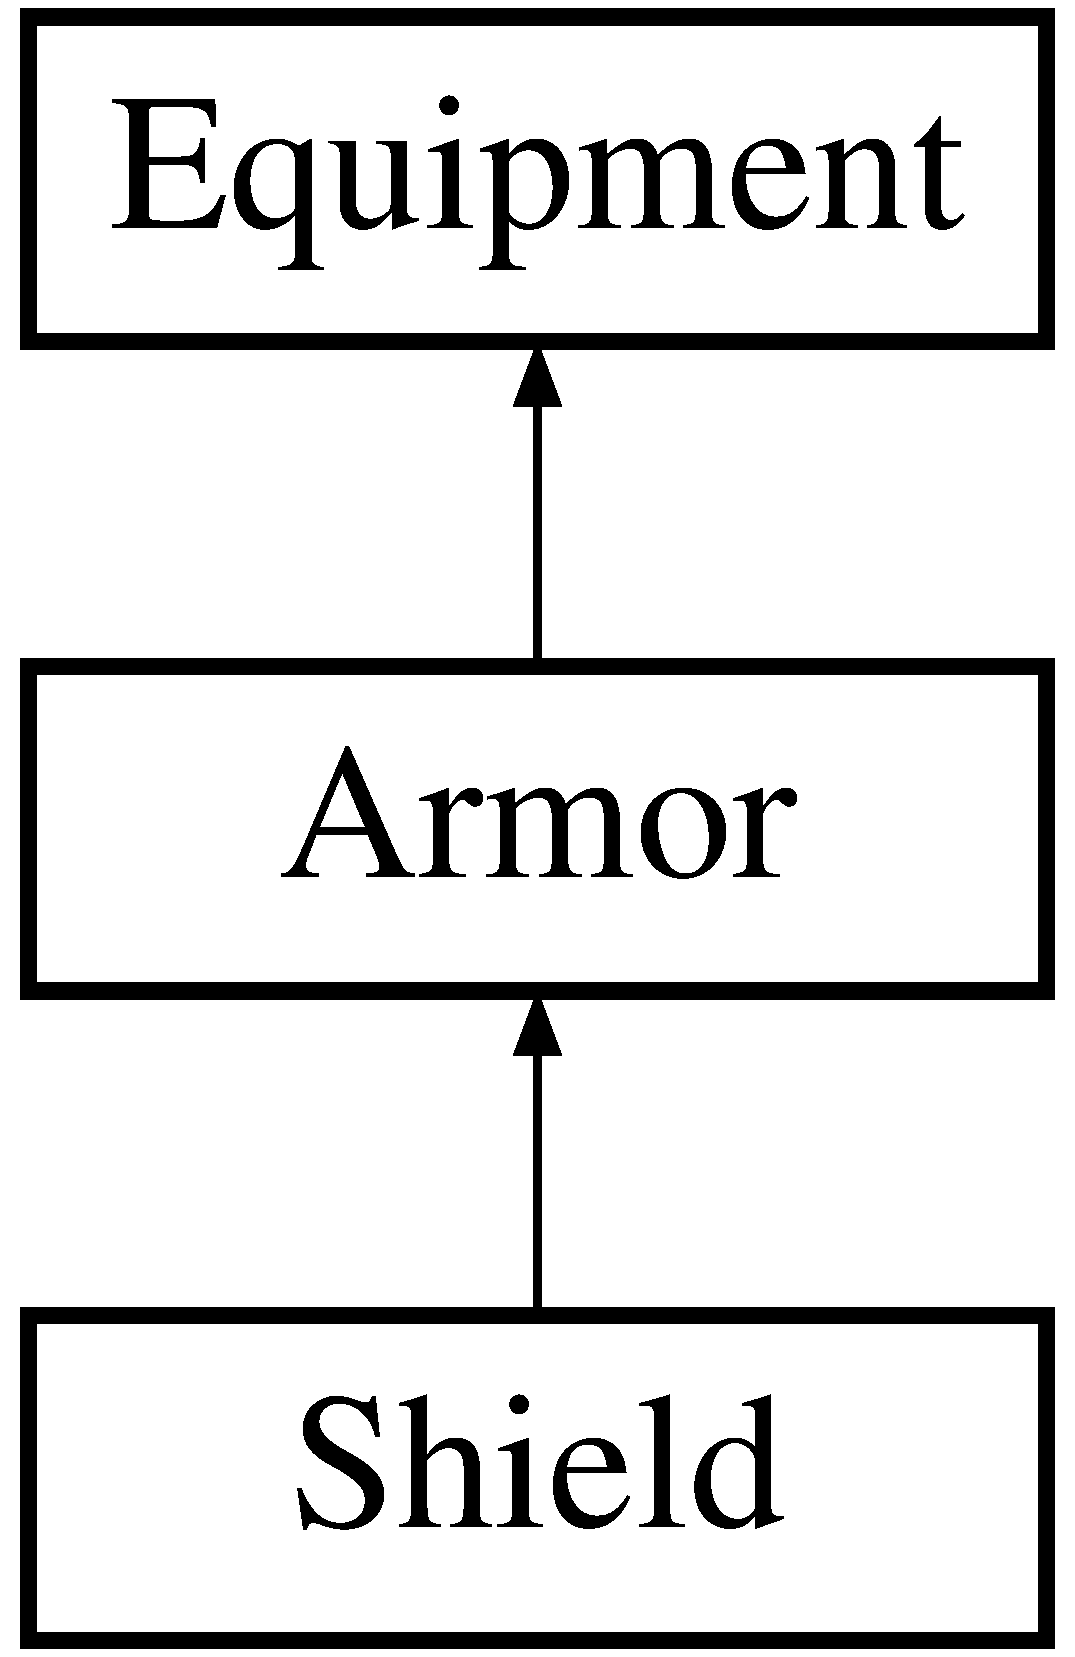
\includegraphics[height=3.000000cm]{class_armor}
\end{center}
\end{figure}
\subsection*{Public Member Functions}
\begin{DoxyCompactItemize}
\item 
\hypertarget{class_armor_a3a8d526767fa5f92fecf3aafd0b97aa7}{}\label{class_armor_a3a8d526767fa5f92fecf3aafd0b97aa7} 
{\bfseries Armor} (string name, int A\+C\+Bonus)
\item 
\hypertarget{class_armor_a83b22277401061f1414a9178994a23c0}{}\label{class_armor_a83b22277401061f1414a9178994a23c0} 
int {\bfseries get\+A\+C\+Bonus} ()
\end{DoxyCompactItemize}


The documentation for this class was generated from the following files\+:\begin{DoxyCompactItemize}
\item 
C\+:/\+Users/\+Sabin-\/\+Laptop/\+Documents/\+Visual Studio 2013/\+Projects/\+Assignment1\+Pr/\+Assignment1\+Pr/Equipment.\+h\item 
C\+:/\+Users/\+Sabin-\/\+Laptop/\+Documents/\+Visual Studio 2013/\+Projects/\+Assignment1\+Pr/\+Assignment1\+Pr/Equipment.\+cpp\end{DoxyCompactItemize}

\hypertarget{class_boots}{}\section{Boots Class Reference}
\label{class_boots}\index{Boots@{Boots}}


Class for boots.  




{\ttfamily \#include $<$Boots.\+h$>$}

Inheritance diagram for Boots\+:\begin{figure}[H]
\begin{center}
\leavevmode
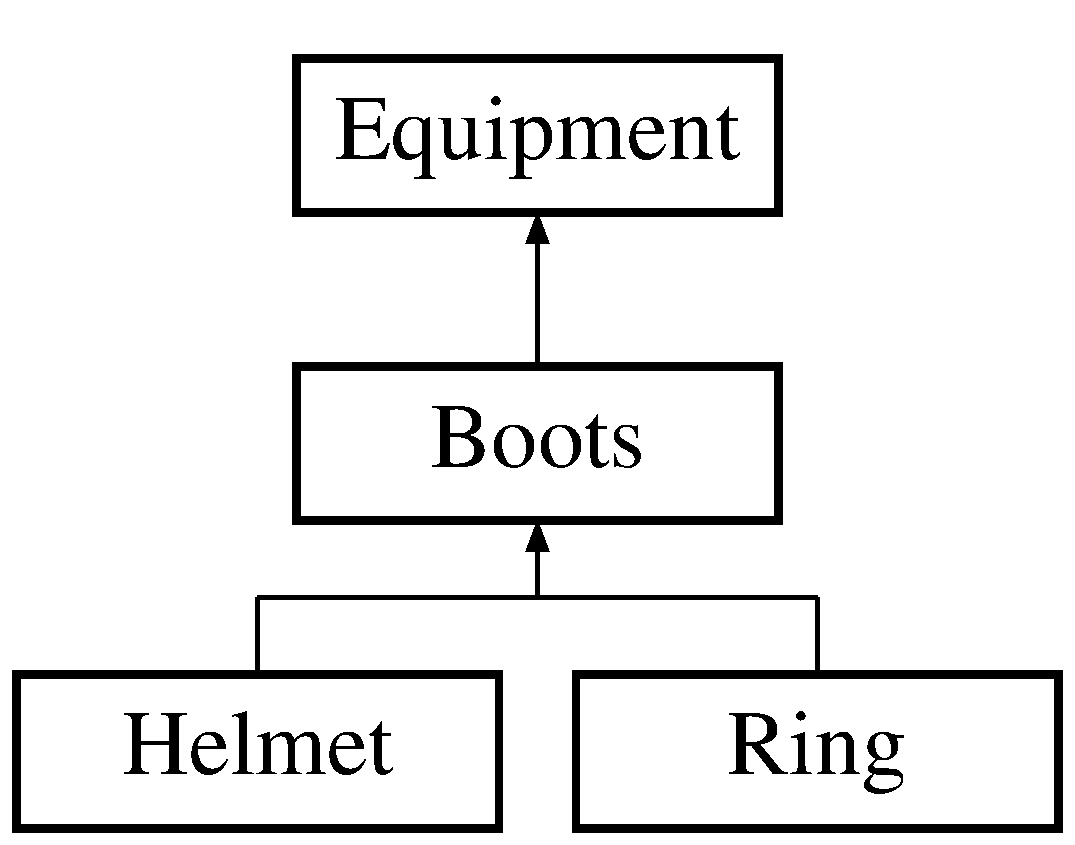
\includegraphics[height=3.000000cm]{class_boots}
\end{center}
\end{figure}
\subsection*{Public Member Functions}
\begin{DoxyCompactItemize}
\item 
\hypertarget{class_boots_abad208e963b53b1f29e269fc246a3485}{}\label{class_boots_abad208e963b53b1f29e269fc246a3485} 
\hyperlink{class_boots_abad208e963b53b1f29e269fc246a3485}{Boots} ()
\begin{DoxyCompactList}\small\item\em Default constructor, useless item as is. \end{DoxyCompactList}\item 
\hyperlink{class_boots_ad3452c78ef60ba4d955e779560d5e5ba}{Boots} (const \hyperlink{class_boots}{Boots} $\ast$other\+Boots)
\item 
\hypertarget{class_boots_adbbf30b0b77d0124262315aeb01647a2}{}\label{class_boots_adbbf30b0b77d0124262315aeb01647a2} 
{\bfseries Boots} (string name, int weight, int value, string \hyperlink{class_item_add84a42b692ee5d580a92ae4a922f784}{image}, array$<$ int, 9 $>$ \hyperlink{class_item_a8532d8729f9433f41b7fc18b20d83236}{enchantment\+Values})
\item 
\hypertarget{class_boots_a04f5b9cfcb60e479cf03321abeebec6d}{}\label{class_boots_a04f5b9cfcb60e479cf03321abeebec6d} 
string \hyperlink{class_boots_a04f5b9cfcb60e479cf03321abeebec6d}{to\+String} ()
\begin{DoxyCompactList}\small\item\em Returns a string with all properties of belt. \end{DoxyCompactList}\end{DoxyCompactItemize}
\subsection*{Protected Member Functions}
\begin{DoxyCompactItemize}
\item 
\hypertarget{class_boots_a067d801af4bd7abb26c9f11970246ed8}{}\label{class_boots_a067d801af4bd7abb26c9f11970246ed8} 
{\bfseries D\+E\+C\+L\+A\+R\+E\+\_\+\+S\+E\+R\+I\+AL} (\hyperlink{class_boots}{Boots})
\end{DoxyCompactItemize}
\subsection*{Additional Inherited Members}


\subsection{Detailed Description}
Class for boots. 

\begin{DoxyAuthor}{Author}
Philip Brink 
\end{DoxyAuthor}
\begin{DoxyVersion}{Version}
0.\+0.\+1 
\end{DoxyVersion}
\begin{DoxyDate}{Date}
2016-\/10-\/20
\end{DoxyDate}
Subclass of \hyperlink{class_item}{Item}, allows Character to equip boots 

\subsection{Constructor \& Destructor Documentation}
\hypertarget{class_boots_ad3452c78ef60ba4d955e779560d5e5ba}{}\label{class_boots_ad3452c78ef60ba4d955e779560d5e5ba} 
\index{Boots@{Boots}!Boots@{Boots}}
\index{Boots@{Boots}!Boots@{Boots}}
\subsubsection{\texorpdfstring{Boots()}{Boots()}}
{\footnotesize\ttfamily Boots\+::\+Boots (\begin{DoxyParamCaption}\item[{const \hyperlink{class_boots}{Boots} $\ast$}]{other\+Boots }\end{DoxyParamCaption})}

Copy-\/constructor -\/ initializes a new pair of boots with the same values as another pair of boots 

The documentation for this class was generated from the following files\+:\begin{DoxyCompactItemize}
\item 
Boots.\+h\item 
Boots.\+cpp\end{DoxyCompactItemize}

\hypertarget{class_characters}{}\section{Characters Class Reference}
\label{class_characters}\index{Characters@{Characters}}


{\ttfamily \#include $<$Characters.\+h$>$}

Inheritance diagram for Characters\+:\begin{figure}[H]
\begin{center}
\leavevmode
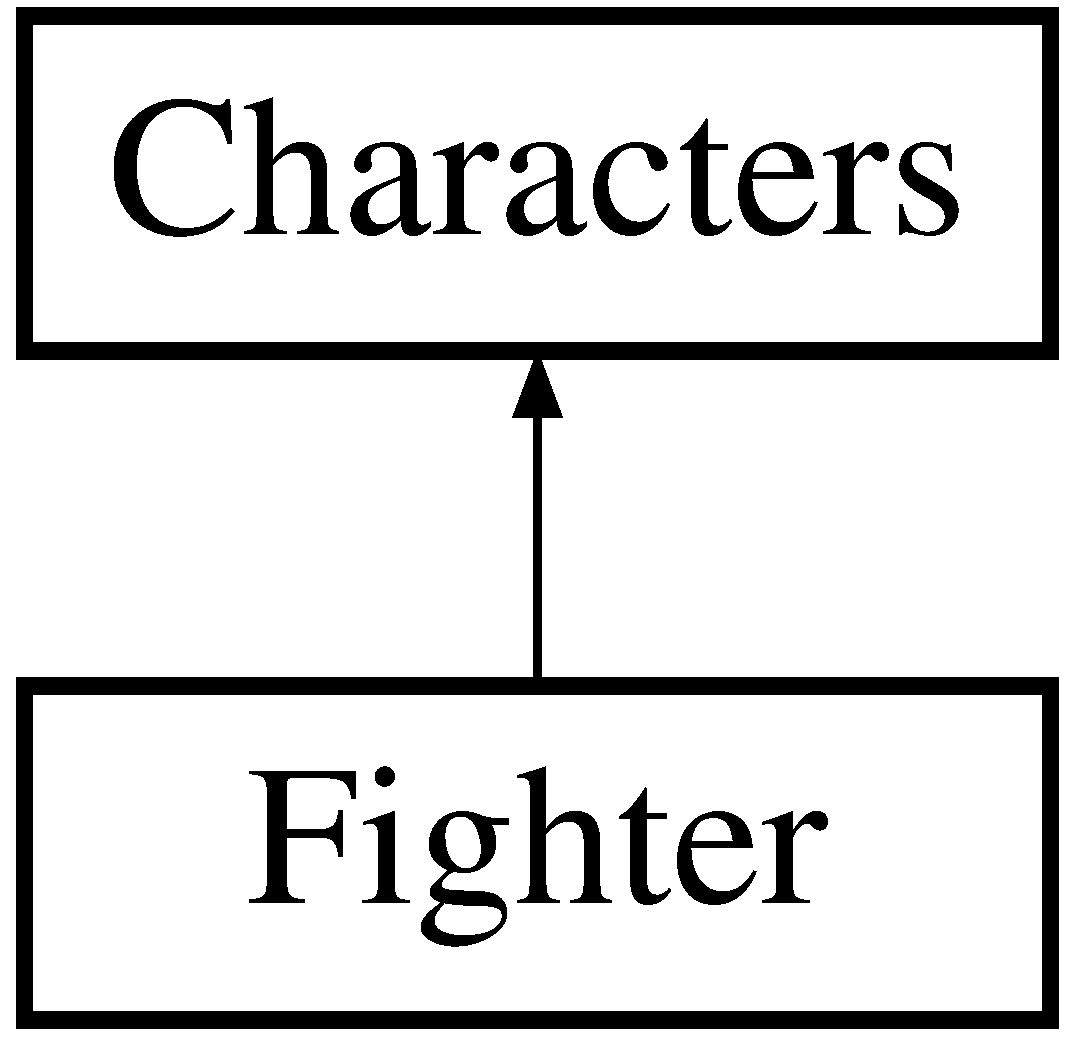
\includegraphics[height=2.000000cm]{class_characters}
\end{center}
\end{figure}
\subsection*{Public Member Functions}
\begin{DoxyCompactItemize}
\item 
\hypertarget{class_characters_a643e74c31b4c20ad614c89e0e046d35f}{}\label{class_characters_a643e74c31b4c20ad614c89e0e046d35f} 
{\bfseries Characters} (int, string)
\item 
\hypertarget{class_characters_a6ec320af5d1526eed47070bca6e4d847}{}\label{class_characters_a6ec320af5d1526eed47070bca6e4d847} 
void {\bfseries destroy\+Object} ()
\item 
\hypertarget{class_characters_a4d7ffd0091e9e37d6da1ad0f0ceaa48f}{}\label{class_characters_a4d7ffd0091e9e37d6da1ad0f0ceaa48f} 
int {\bfseries get\+Level} ()
\item 
\hypertarget{class_characters_a498fb8e0caaa6503fbb1e1694a082c4c}{}\label{class_characters_a498fb8e0caaa6503fbb1e1694a082c4c} 
int {\bfseries get\+Scores} (int, int)
\item 
\hypertarget{class_characters_adc5a2d1c1aabab2b9915f5ce0e2707f9}{}\label{class_characters_adc5a2d1c1aabab2b9915f5ce0e2707f9} 
void {\bfseries display\+Stats} ()
\item 
\hypertarget{class_characters_acf1c5f4228c0ac33361c0ad5211aa7a9}{}\label{class_characters_acf1c5f4228c0ac33361c0ad5211aa7a9} 
void {\bfseries display\+Equip} ()
\item 
\hypertarget{class_characters_afa9c56654b160d186ce3fd8259f8f180}{}\label{class_characters_afa9c56654b160d186ce3fd8259f8f180} 
int {\bfseries roll\+Dice} (int)
\item 
\hypertarget{class_characters_aef7eb04814a81a6043dad4033954e4ad}{}\label{class_characters_aef7eb04814a81a6043dad4033954e4ad} 
void {\bfseries equip} (\hyperlink{class_armor}{Armor} $\ast$)
\item 
\hypertarget{class_characters_a1f334afbb902a822bbb308634683a1a4}{}\label{class_characters_a1f334afbb902a822bbb308634683a1a4} 
void {\bfseries equip} (\hyperlink{class_weapon}{Weapon} $\ast$)
\item 
\hypertarget{class_characters_a5626b3e730753e2da255debb2c692011}{}\label{class_characters_a5626b3e730753e2da255debb2c692011} 
void {\bfseries equip} (\hyperlink{class_helmet}{Helmet} $\ast$)
\item 
\hypertarget{class_characters_a65af5ec102b0bfb39cdd84d6471f8529}{}\label{class_characters_a65af5ec102b0bfb39cdd84d6471f8529} 
void {\bfseries equip} (\hyperlink{class_boots}{Boots} $\ast$)
\item 
\hypertarget{class_characters_a865239b8e8826d1213862897061ed718}{}\label{class_characters_a865239b8e8826d1213862897061ed718} 
void {\bfseries equip} (\hyperlink{class_ring}{Ring} $\ast$)
\item 
\hypertarget{class_characters_a5baae929baa10ce365efc64bd3bcea88}{}\label{class_characters_a5baae929baa10ce365efc64bd3bcea88} 
void {\bfseries equip} (\hyperlink{class_shield}{Shield} $\ast$)
\item 
\hypertarget{class_characters_ab2ff7cf1e6a50e005396ac7ff29c6dad}{}\label{class_characters_ab2ff7cf1e6a50e005396ac7ff29c6dad} 
string {\bfseries current\+Armor} ()
\item 
\hypertarget{class_characters_adf56654d23486d7779a006a0b5ed156e}{}\label{class_characters_adf56654d23486d7779a006a0b5ed156e} 
string {\bfseries current\+Weapon} ()
\item 
\hypertarget{class_characters_a1e4c32972619f14dbeae485316f77a5d}{}\label{class_characters_a1e4c32972619f14dbeae485316f77a5d} 
string {\bfseries current\+Shield} ()
\item 
\hypertarget{class_characters_a26db054e9899a900b62d105d5bf2b20c}{}\label{class_characters_a26db054e9899a900b62d105d5bf2b20c} 
string {\bfseries current\+Helmet} ()
\item 
\hypertarget{class_characters_a9f6a49663aceb01d8a5391d75482a224}{}\label{class_characters_a9f6a49663aceb01d8a5391d75482a224} 
string {\bfseries current\+Boots} ()
\item 
\hypertarget{class_characters_a02fd5bc3c6122b602d6aaf329a8cdaba}{}\label{class_characters_a02fd5bc3c6122b602d6aaf329a8cdaba} 
string {\bfseries current\+Ring} ()
\item 
bool \hyperlink{class_characters_a1273e2d7fe2e959cd3ed513c5717f6b7}{validate\+New\+Character} ()
\begin{DoxyCompactList}\small\item\em F\+OR U\+N\+IT T\+E\+ST. \end{DoxyCompactList}\item 
\hypertarget{class_characters_a8a13cb967bd25662f86eac505e3e874a}{}\label{class_characters_a8a13cb967bd25662f86eac505e3e874a} 
bool {\bfseries validate\+Proficiency} ()
\end{DoxyCompactItemize}


\subsection{Detailed Description}
This class is used to create a general character.

All characters are created with a level and a name. Once this is given, the amount of experience and proficiency bonus are determine by the level.

All characters have 6 ability scores and their corresponding modifiers. Modifiers are calculated using the formula floor((score-\/10)/2). Ability scores are randomly generated using a 4\+D6 dice roll and taking the 3 largest values and adding them together. Then the highest is set to S\+TR and the second highest to C\+ON, while all others remain arbitrary.

The armor class is dependent on the equipment of the character. By default, all characters with Level 1 will only have a \char`\"{}\+Longsword\char`\"{} equipped while all others will be in posession of a \char`\"{}\+Light Crossbow\char`\"{} and \char`\"{}\+Padded Armor\char`\"{} for armor. If no armor is worn, AC = 10 + C\+O\+N\+\_\+\+Mod + A\+C\+\_\+\+Bonuses where A\+C\+\_\+\+Bonuses can be from shield, helmet, boots, and ring. (if the three last ones have a bonus type of AC) If armor is worn, AC = Armor\+\_\+\+Bonus + C\+O\+N\+\_\+\+Mod + A\+C\+\_\+\+Bonuses

Lastly the Attack Bonus and Damage Bonus are dependent on the type of weapon in use.

Attack\+\_\+\+Bonus = Proficiency\+\_\+\+Bonus + (S\+T\+R\+\_\+\+Mod or D\+E\+X\+\_\+\+Mod) and Damage\+\_\+\+Bonus = (S\+T\+R\+\_\+\+Mod or D\+E\+X\+\_\+\+Mod)

If the weapon is a melee weapon, S\+T\+R\+\_\+\+Mod is used in the above equations, if ranged, D\+E\+X\+\_\+\+Mod is used

In addition all characters may equip an \hyperlink{class_armor}{Armor}, \hyperlink{class_weapon}{Weapon}, \hyperlink{class_boots}{Boots}, \hyperlink{class_ring}{Ring}, \hyperlink{class_helmet}{Helmet} and \hyperlink{class_shield}{Shield}. When equipping new equipment, the character stats are adjusted to remove whatever effect they had if applicable or recalculate AC. M\+O\+RE I\+N\+F\+O\+R\+M\+A\+T\+I\+ON A\+B\+O\+UT T\+H\+IS IN E\+Q\+U\+I\+P\+M\+E\+NT C\+L\+A\+SS 

\subsection{Member Function Documentation}
\hypertarget{class_characters_a1273e2d7fe2e959cd3ed513c5717f6b7}{}\label{class_characters_a1273e2d7fe2e959cd3ed513c5717f6b7} 
\index{Characters@{Characters}!validate\+New\+Character@{validate\+New\+Character}}
\index{validate\+New\+Character@{validate\+New\+Character}!Characters@{Characters}}
\subsubsection{\texorpdfstring{validate\+New\+Character()}{validateNewCharacter()}}
{\footnotesize\ttfamily bool Characters\+::validate\+New\+Character (\begin{DoxyParamCaption}{ }\end{DoxyParamCaption})}



F\+OR U\+N\+IT T\+E\+ST. 

Check to see if score values are valid (3 to 18) 

The documentation for this class was generated from the following files\+:\begin{DoxyCompactItemize}
\item 
C\+:/\+Users/\+Sabin-\/\+Laptop/\+Documents/\+Visual Studio 2013/\+Projects/\+Assignment1\+Pr/\+Assignment1\+Pr/Characters.\+h\item 
C\+:/\+Users/\+Sabin-\/\+Laptop/\+Documents/\+Visual Studio 2013/\+Projects/\+Assignment1\+Pr/\+Assignment1\+Pr/Characters.\+cpp\end{DoxyCompactItemize}

\hypertarget{class_equipment}{}\section{Equipment Class Reference}
\label{class_equipment}\index{Equipment@{Equipment}}


{\ttfamily \#include $<$Equipment.\+h$>$}

Inheritance diagram for Equipment\+:\begin{figure}[H]
\begin{center}
\leavevmode
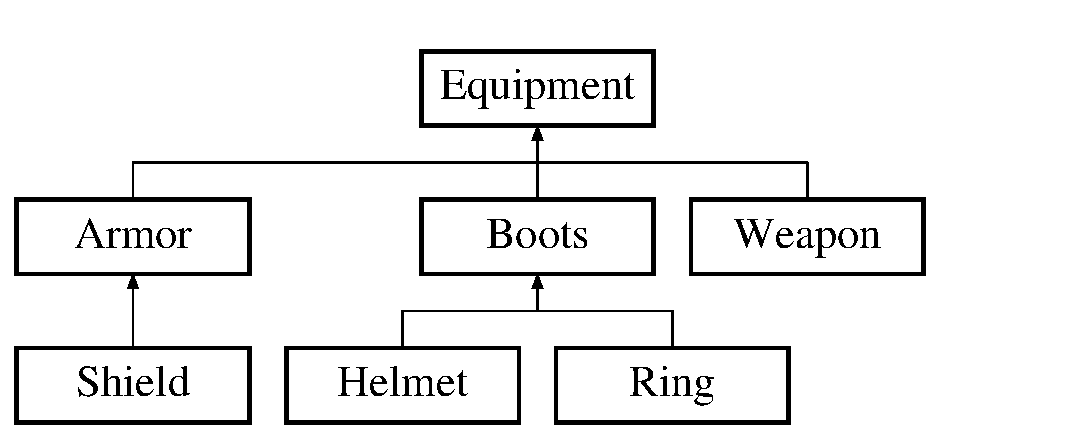
\includegraphics[height=3.000000cm]{class_equipment}
\end{center}
\end{figure}
\subsection*{Public Member Functions}
\begin{DoxyCompactItemize}
\item 
\hypertarget{class_equipment_a40b66c38f62cee0ef51b7062d91946bf}{}\label{class_equipment_a40b66c38f62cee0ef51b7062d91946bf} 
{\bfseries Equipment} (string name)
\item 
\hypertarget{class_equipment_abfde2b1761f374597f0efbfbf44b28a3}{}\label{class_equipment_abfde2b1761f374597f0efbfbf44b28a3} 
string {\bfseries get\+Name} ()
\item 
\hypertarget{class_equipment_ad1fe2caf19e8f5c2d7a20610b0aa048b}{}\label{class_equipment_ad1fe2caf19e8f5c2d7a20610b0aa048b} 
bool {\bfseries compare\+Name} (string name)
\end{DoxyCompactItemize}


\subsection{Detailed Description}
This class is a dummy class to implement equipments. All equipment have names but each type of equipment has different affects on character stats depending on the type of equipment and bonus types they implement.

All armors inherit from \hyperlink{class_equipment}{Equipment} and have an A\+C\+Bonus.

All shields inherit from Armors since they also only have an A\+C\+Bonus.

All weapons inherit from \hyperlink{class_equipment}{Equipment} and have a dieroll and a type (melee or ranged)

All boots inherit from \hyperlink{class_equipment}{Equipment} and have a bonustype and a bonus value. Bonustypes are as follows\+: 0 = N\+O\+NE, 1 = D\+EX, 2 = AC

All helmets inherit from \hyperlink{class_boots}{Boots} and also have a bonustype and bonus value. Bonustypes are as follows\+: 0 = N\+O\+NE, 1 = I\+NT, 2 = W\+IS, 3 = AC

All rings inherit from \hyperlink{class_boots}{Boots} and also have a bonustype and bonus value. Bonustypes are as follows\+: 0 = N\+O\+NE, 1= S\+TR, 2 = C\+ON, 3 = W\+IS, 4 = C\+HA, 5 = AC

N\+O\+TE\+: name is set to \char`\"{}\+N\+O\+N\+E\char`\"{} when using the default constructor. Therefore, to de-\/equip, simply call the default constructor of any equipment type. This will set all values to 0 or empty string. 

The documentation for this class was generated from the following files\+:\begin{DoxyCompactItemize}
\item 
C\+:/\+Users/\+Sabin-\/\+Laptop/\+Documents/\+Visual Studio 2013/\+Projects/\+Assignment1\+Pr/\+Assignment1\+Pr/Equipment.\+h\item 
C\+:/\+Users/\+Sabin-\/\+Laptop/\+Documents/\+Visual Studio 2013/\+Projects/\+Assignment1\+Pr/\+Assignment1\+Pr/Equipment.\+cpp\end{DoxyCompactItemize}

\hypertarget{class_fighter}{}\section{Fighter Class Reference}
\label{class_fighter}\index{Fighter@{Fighter}}


Provides resource for management of \hyperlink{class_fighter}{Fighter} within game.  




{\ttfamily \#include $<$Fighter.\+h$>$}

Inheritance diagram for Fighter\+:\begin{figure}[H]
\begin{center}
\leavevmode
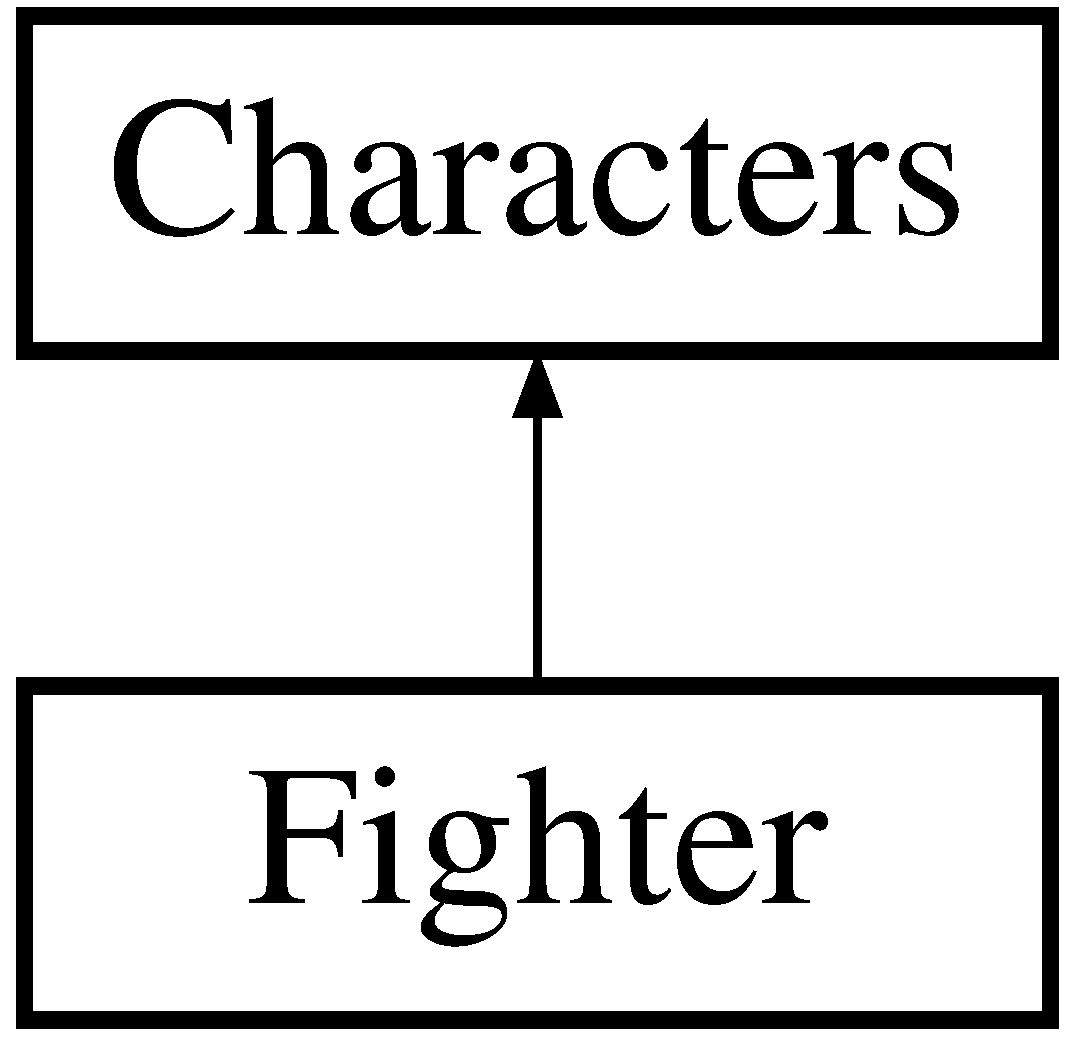
\includegraphics[height=3.000000cm]{class_fighter}
\end{center}
\end{figure}
\subsection*{Public Member Functions}
\begin{DoxyCompactItemize}
\item 
\hypertarget{class_fighter_ad1fcbd2f4c389221611e379f3df46ca8}{}\label{class_fighter_ad1fcbd2f4c389221611e379f3df46ca8} 
\hyperlink{class_fighter_ad1fcbd2f4c389221611e379f3df46ca8}{Fighter} (int, \hyperlink{_entity_8h_aa2df4028f474807638d438104900b003}{Race}, string)
\begin{DoxyCompactList}\small\item\em Parameterized Constructor to set level, race and name. \end{DoxyCompactList}\item 
\hypertarget{class_fighter_a601ebcca9ea2287c54a0995dc11a117c}{}\label{class_fighter_a601ebcca9ea2287c54a0995dc11a117c} 
\hyperlink{class_fighter_a601ebcca9ea2287c54a0995dc11a117c}{Fighter} (int level, \hyperlink{_entity_8h_aa2df4028f474807638d438104900b003}{Race} race, string name, int S\+TR, int D\+EX, int C\+ON, int I\+NT, int W\+IS, int C\+HA)
\begin{DoxyCompactList}\small\item\em Parameterized constructor to set all att of \hyperlink{class_fighter}{Fighter}. \end{DoxyCompactList}\item 
\hypertarget{class_fighter_a5bfd7630b47d4bf3b7b1288195bbad07}{}\label{class_fighter_a5bfd7630b47d4bf3b7b1288195bbad07} 
void \hyperlink{class_fighter_a5bfd7630b47d4bf3b7b1288195bbad07}{init\+Hit\+Points} ()
\begin{DoxyCompactList}\small\item\em Function that calculates the initial hitpoints of the character based on the level. \end{DoxyCompactList}\item 
\hypertarget{class_fighter_a82d21934022da1ffe16396e5fb407897}{}\label{class_fighter_a82d21934022da1ffe16396e5fb407897} 
void \hyperlink{class_fighter_a82d21934022da1ffe16396e5fb407897}{recalc\+Hit\+Points} ()
\begin{DoxyCompactList}\small\item\em Function to recalculate hitpoints when leveling up but adding a roll of hit\+Dice and dexterity modifier. \end{DoxyCompactList}\item 
\hypertarget{class_fighter_a9e63e29c35aaca0bc60ee46efe00cc62}{}\label{class_fighter_a9e63e29c35aaca0bc60ee46efe00cc62} 
void \hyperlink{class_fighter_a9e63e29c35aaca0bc60ee46efe00cc62}{display\+Stats} ()
\begin{DoxyCompactList}\small\item\em Function to displays the fighter stats, calls parent \hyperlink{class_fighter_a9e63e29c35aaca0bc60ee46efe00cc62}{display\+Stats()} \end{DoxyCompactList}\item 
\hypertarget{class_fighter_ad519375531d2f4ae2bc8896e3595d5f4}{}\label{class_fighter_ad519375531d2f4ae2bc8896e3595d5f4} 
void \hyperlink{class_fighter_ad519375531d2f4ae2bc8896e3595d5f4}{display\+Battle} ()
\begin{DoxyCompactList}\small\item\em Function to display fighter battle stats, calls parent \hyperlink{class_fighter_ad519375531d2f4ae2bc8896e3595d5f4}{display\+Battle()} \end{DoxyCompactList}\item 
\hypertarget{class_fighter_afa53e25a50772d86c5e929c6df1354ad}{}\label{class_fighter_afa53e25a50772d86c5e929c6df1354ad} 
void \hyperlink{class_fighter_afa53e25a50772d86c5e929c6df1354ad}{display\+Level\+Up} ()
\begin{DoxyCompactList}\small\item\em Function to display fighter stats when leveling up, calls parent \hyperlink{class_fighter_afa53e25a50772d86c5e929c6df1354ad}{display\+Level\+Up()} \end{DoxyCompactList}\item 
\hypertarget{class_fighter_a6a050f0b907517b09627fe16cea6e341}{}\label{class_fighter_a6a050f0b907517b09627fe16cea6e341} 
void \hyperlink{class_fighter_a6a050f0b907517b09627fe16cea6e341}{display\+Death} ()
\begin{DoxyCompactList}\small\item\em Function to display fighter\textquotesingle{}s death, calls parent \hyperlink{class_fighter_afa53e25a50772d86c5e929c6df1354ad}{display\+Level\+Up()} and terminates the program. \end{DoxyCompactList}\item 
\hypertarget{class_fighter_abf4d82d4a17d37d3b5ca4084debabde4}{}\label{class_fighter_abf4d82d4a17d37d3b5ca4084debabde4} 
string \hyperlink{class_fighter_abf4d82d4a17d37d3b5ca4084debabde4}{get\+Name} ()
\begin{DoxyCompactList}\small\item\em Returns name of \hyperlink{class_fighter}{Fighter}. \end{DoxyCompactList}\item 
\hypertarget{class_fighter_a2a733caf375a8d2e1c514418267e5017}{}\label{class_fighter_a2a733caf375a8d2e1c514418267e5017} 
\hyperlink{_entity_8h_aa2df4028f474807638d438104900b003}{Race} \hyperlink{class_fighter_a2a733caf375a8d2e1c514418267e5017}{get\+Race} ()
\begin{DoxyCompactList}\small\item\em Returns race. \end{DoxyCompactList}\item 
void \hyperlink{class_fighter_af692d6c9b24f902c13bb8b7f3350631e}{set\+Name} (string name)
\begin{DoxyCompactList}\small\item\em Sets name. \end{DoxyCompactList}\item 
void \hyperlink{class_fighter_abd0aa443cda40a70c7df3bf1949a9e79}{set\+Race} (\hyperlink{_entity_8h_aa2df4028f474807638d438104900b003}{Race} n\+Race)
\begin{DoxyCompactList}\small\item\em Sets Race. \end{DoxyCompactList}\item 
void \hyperlink{class_fighter_ac1a886e2f60333e38e90fff2a0f6107b}{attack} (\hyperlink{class_monster}{Monster} $\ast$c)
\item 
void \hyperlink{class_fighter_afe019dbd9ed0f0d10e047127dc478a63}{receive\+Damage} (int)
\item 
\hypertarget{class_fighter_a886a5fe6b7579951e64e68b76482b29c}{}\label{class_fighter_a886a5fe6b7579951e64e68b76482b29c} 
void \hyperlink{class_fighter_a886a5fe6b7579951e64e68b76482b29c}{level\+Up} (int)
\begin{DoxyCompactList}\small\item\em Function for level up processing to increment chosen ability score and recalculates hitpoints. \end{DoxyCompactList}\item 
void \hyperlink{class_fighter_af411947929c37ef0a0eab87b0c45f4f3}{gain\+Experience} (int)
\item 
\hypertarget{class_fighter_af690e4afec50a9c446120db47b463d84}{}\label{class_fighter_af690e4afec50a9c446120db47b463d84} 
void {\bfseries dead} ()
\item 
\hypertarget{class_fighter_ae888de59ae299553890387c58d774bda}{}\label{class_fighter_ae888de59ae299553890387c58d774bda} 
void {\bfseries current\+State} ()
\item 
\hypertarget{class_fighter_a60976eb2c11504befe0aff8522339636}{}\label{class_fighter_a60976eb2c11504befe0aff8522339636} 
void \hyperlink{class_fighter_a60976eb2c11504befe0aff8522339636}{equip\+Options} ()
\begin{DoxyCompactList}\small\item\em Function to display when player will equip-\/dequip equipment. \end{DoxyCompactList}\item 
void \hyperlink{class_fighter_acabd4955401ddf3ddc0be5f28fa64267}{equip\+Armor} (int i)
\item 
void \hyperlink{class_fighter_a4d88916d33514e2c7e5aaaef8916f93c}{equip\+Weapon} (int i)
\item 
void \hyperlink{class_fighter_ae90d7de8a4d6b61b35f43cefe7ec940c}{equip\+Helmet} (int i)
\item 
\hypertarget{class_fighter_aabfc72ac049b808fabbb77aa9fdfcba4}{}\label{class_fighter_aabfc72ac049b808fabbb77aa9fdfcba4} 
void \hyperlink{class_fighter_aabfc72ac049b808fabbb77aa9fdfcba4}{equip\+Boots} (int i)
\begin{DoxyCompactList}\small\item\em Function to equip boots. Previous bonus is removed and recalculate the bonus based on new boots. Triggers redisplay of stats. \end{DoxyCompactList}\item 
\hypertarget{class_fighter_a51cff2d6b9af41b0f6a2ca3a26b6eb42}{}\label{class_fighter_a51cff2d6b9af41b0f6a2ca3a26b6eb42} 
void \hyperlink{class_fighter_a51cff2d6b9af41b0f6a2ca3a26b6eb42}{equip\+Ring} (int i)
\begin{DoxyCompactList}\small\item\em Function to equip ring. Previous bonus is removed and recalculate the bonus based on new ring. Triggers redisplay of stats. \end{DoxyCompactList}\item 
\hypertarget{class_fighter_af314de4ade8520638065735f2ebd3fc8}{}\label{class_fighter_af314de4ade8520638065735f2ebd3fc8} 
void \hyperlink{class_fighter_af314de4ade8520638065735f2ebd3fc8}{equip\+Shield} (int i)
\begin{DoxyCompactList}\small\item\em Function to equip shield. Previous AC bonus is removed and recalculate the AC based on new shield. Triggers redisplay of stats. \end{DoxyCompactList}\item 
\hypertarget{class_fighter_aed08492ff6120638f476309a50887841}{}\label{class_fighter_aed08492ff6120638f476309a50887841} 
void \hyperlink{class_fighter_aed08492ff6120638f476309a50887841}{equip\+Belt} (int i)
\begin{DoxyCompactList}\small\item\em Function to equip belt. Previous bonuses are removed. Triggers redisplay of stats. \end{DoxyCompactList}\item 
bool \hyperlink{class_fighter_a69dccfbc61abf5720e8a329203158d1e}{pickup\+Item} (\hyperlink{class_item}{Item} $\ast$i)
\item 
bool \hyperlink{class_fighter_a572fb61d329f4993701900ff3a1db5f8}{fill\+Backpack} (\hyperlink{class_container}{Container} $\ast$other\+Container)
\item 
bool \hyperlink{class_fighter_a66c0adfa4979fa3ac994359a188121a8}{interact\+With\+Container} (\hyperlink{class_container}{Container} $\ast$the\+Container)
\item 
\hypertarget{class_fighter_ac7a95f5d4b59bca227f847924625ffc2}{}\label{class_fighter_ac7a95f5d4b59bca227f847924625ffc2} 
void \hyperlink{class_fighter_ac7a95f5d4b59bca227f847924625ffc2}{deequip\+Armor} ()
\begin{DoxyCompactList}\small\item\em Function to de-\/equip Armor(). Resets stats and puts armor in backpack, as long as there is space. \end{DoxyCompactList}\item 
\hypertarget{class_fighter_a277fd0526a0318923f2775356f30972f}{}\label{class_fighter_a277fd0526a0318923f2775356f30972f} 
void \hyperlink{class_fighter_a277fd0526a0318923f2775356f30972f}{dequip\+Weapon} ()
\begin{DoxyCompactList}\small\item\em Function to de-\/equip \hyperlink{class_weapon}{Weapon}. Resets stats and puts weapon in backpack, as long as there is space. \end{DoxyCompactList}\item 
\hypertarget{class_fighter_a9e6f83324d66e6467d8af19e91c13781}{}\label{class_fighter_a9e6f83324d66e6467d8af19e91c13781} 
void \hyperlink{class_fighter_a9e6f83324d66e6467d8af19e91c13781}{deequip\+Helmet} ()
\begin{DoxyCompactList}\small\item\em Function to de-\/equip \hyperlink{class_helmet}{Helmet}. Resets stats and puts helmet in backpack, as long as there is space. \end{DoxyCompactList}\item 
\hypertarget{class_fighter_add80df04f0659d37c0e30e91314e3d5e}{}\label{class_fighter_add80df04f0659d37c0e30e91314e3d5e} 
void \hyperlink{class_fighter_add80df04f0659d37c0e30e91314e3d5e}{deequip\+Boots} ()
\begin{DoxyCompactList}\small\item\em Function to de-\/equip \hyperlink{class_boots}{Boots}. Resets stats and puts boots in backpack, as long as there is space. \end{DoxyCompactList}\item 
\hypertarget{class_fighter_a1b64aab99d09a1d9a31b8674b4d0176c}{}\label{class_fighter_a1b64aab99d09a1d9a31b8674b4d0176c} 
void \hyperlink{class_fighter_a1b64aab99d09a1d9a31b8674b4d0176c}{deequip\+Ring} ()
\begin{DoxyCompactList}\small\item\em Function to de-\/equip \hyperlink{class_ring}{Ring}. Resets stats and puts ring in backpack, as long as there is space. \end{DoxyCompactList}\item 
\hypertarget{class_fighter_a313e661908412be41e7f3f67c3c050f4}{}\label{class_fighter_a313e661908412be41e7f3f67c3c050f4} 
void \hyperlink{class_fighter_a313e661908412be41e7f3f67c3c050f4}{deequip\+Shield} ()
\begin{DoxyCompactList}\small\item\em Function to de-\/equip \hyperlink{class_shield}{Shield}. Resets stats and puts shield in backpack, as long as there is space. \end{DoxyCompactList}\item 
\hypertarget{class_fighter_a529fdd57ee79c761a7601356f861d7fb}{}\label{class_fighter_a529fdd57ee79c761a7601356f861d7fb} 
void \hyperlink{class_fighter_a529fdd57ee79c761a7601356f861d7fb}{deequip\+Belt} ()
\begin{DoxyCompactList}\small\item\em Function to de-\/equip belt. Resets stats and puts belt in backpack, as long as there is space. \end{DoxyCompactList}\item 
\hypertarget{class_fighter_a30734efb2140029276fd7528d28685fc}{}\label{class_fighter_a30734efb2140029276fd7528d28685fc} 
void \hyperlink{class_fighter_a30734efb2140029276fd7528d28685fc}{display\+Equiped} ()
\begin{DoxyCompactList}\small\item\em Function to equip armor. Previous AC bonus is removed and recalculate the AC based on new armor. Triggers redisplay of stats. \end{DoxyCompactList}\item 
\hypertarget{class_fighter_a1f026b1314d058a8033a19328a40e4cb}{}\label{class_fighter_a1f026b1314d058a8033a19328a40e4cb} 
void {\bfseries display\+Backpack} ()
\item 
void \hyperlink{class_fighter_a5dd8b95b965832bbae65d6285a9bac53}{display\+Only\+Stats} ()
\item 
\hypertarget{class_fighter_a235df759d42bb20bd6314abe806dd6ce}{}\label{class_fighter_a235df759d42bb20bd6314abe806dd6ce} 
bool {\bfseries validate\+Hit\+Points} ()
\item 
\hypertarget{class_fighter_a7372ff74df453241ee2d990a265fd71c}{}\label{class_fighter_a7372ff74df453241ee2d990a265fd71c} 
bool \hyperlink{class_fighter_a7372ff74df453241ee2d990a265fd71c}{validate\+Death} ()
\begin{DoxyCompactList}\small\item\em test function to validate character death \end{DoxyCompactList}\item 
\hypertarget{class_fighter_a05f927eea7af56811cce5a8ba2c8a349}{}\label{class_fighter_a05f927eea7af56811cce5a8ba2c8a349} 
bool {\bfseries validate\+Gain\+Experience} (int)
\item 
\hypertarget{class_fighter_a66d147cbc9c3690009cad90a6ee35f42}{}\label{class_fighter_a66d147cbc9c3690009cad90a6ee35f42} 
bool {\bfseries validate\+Map\+Component\+Within\+Range} (int x, int y)
\item 
bool \hyperlink{class_fighter_ab2a750803d7df7f1d66e9b40074f7a41}{validate\+Player\+Move} (int x, int y)
\item 
virtual void \hyperlink{class_fighter_a44b8e8e71e55b645c4fe7f67ef844e87}{Serialize} (C\+Archive \&ar)
\end{DoxyCompactItemize}
\subsection*{Protected Member Functions}
\begin{DoxyCompactItemize}
\item 
\hypertarget{class_fighter_a349455a2930ba35778477b876c5ea0eb}{}\label{class_fighter_a349455a2930ba35778477b876c5ea0eb} 
{\bfseries D\+E\+C\+L\+A\+R\+E\+\_\+\+S\+E\+R\+I\+AL} (\hyperlink{class_fighter}{Fighter})
\end{DoxyCompactItemize}
\subsection*{Additional Inherited Members}


\subsection{Detailed Description}
Provides resource for management of \hyperlink{class_fighter}{Fighter} within game. 

Subclass of \hyperlink{class_characters}{Characters}, \textquotesingle{}\hyperlink{class_fighter}{Fighter}\textquotesingle{} character class implementation 

\subsection{Member Function Documentation}
\hypertarget{class_fighter_ac1a886e2f60333e38e90fff2a0f6107b}{}\label{class_fighter_ac1a886e2f60333e38e90fff2a0f6107b} 
\index{Fighter@{Fighter}!attack@{attack}}
\index{attack@{attack}!Fighter@{Fighter}}
\subsubsection{\texorpdfstring{attack()}{attack()}}
{\footnotesize\ttfamily void Fighter\+::attack (\begin{DoxyParamCaption}\item[{\hyperlink{class_monster}{Monster} $\ast$}]{c }\end{DoxyParamCaption})}

Function for attacking a \hyperlink{class_monster}{Monster}, generates attack roll and checks it agains \hyperlink{class_monster}{Monster}\textquotesingle{}s AC If larger than AC, damage roll is calculated and inflicted on \hyperlink{class_monster}{Monster}, otherwise attack fails \hypertarget{class_fighter_a5dd8b95b965832bbae65d6285a9bac53}{}\label{class_fighter_a5dd8b95b965832bbae65d6285a9bac53} 
\index{Fighter@{Fighter}!display\+Only\+Stats@{display\+Only\+Stats}}
\index{display\+Only\+Stats@{display\+Only\+Stats}!Fighter@{Fighter}}
\subsubsection{\texorpdfstring{display\+Only\+Stats()}{displayOnlyStats()}}
{\footnotesize\ttfamily void Fighter\+::display\+Only\+Stats (\begin{DoxyParamCaption}{ }\end{DoxyParamCaption})}

Displays only the stats of the \hyperlink{class_fighter}{Fighter}, does not provide ability to edit inventory \hypertarget{class_fighter_acabd4955401ddf3ddc0be5f28fa64267}{}\label{class_fighter_acabd4955401ddf3ddc0be5f28fa64267} 
\index{Fighter@{Fighter}!equip\+Armor@{equip\+Armor}}
\index{equip\+Armor@{equip\+Armor}!Fighter@{Fighter}}
\subsubsection{\texorpdfstring{equip\+Armor()}{equipArmor()}}
{\footnotesize\ttfamily void Fighter\+::equip\+Armor (\begin{DoxyParamCaption}\item[{int}]{i }\end{DoxyParamCaption})}

Allows the \hyperlink{class_fighter}{Fighter} to equip piece of armor at index \textquotesingle{}i\textquotesingle{} in the backpack. If no armor is equipped, then nothing special happens. If the \hyperlink{class_fighter}{Fighter} already has armor equipped, then it is returned to the backpack. 
\begin{DoxyParams}{Parameters}
{\em i} & index of armor in background \\
\hline
\end{DoxyParams}
\hypertarget{class_fighter_ae90d7de8a4d6b61b35f43cefe7ec940c}{}\label{class_fighter_ae90d7de8a4d6b61b35f43cefe7ec940c} 
\index{Fighter@{Fighter}!equip\+Helmet@{equip\+Helmet}}
\index{equip\+Helmet@{equip\+Helmet}!Fighter@{Fighter}}
\subsubsection{\texorpdfstring{equip\+Helmet()}{equipHelmet()}}
{\footnotesize\ttfamily void Fighter\+::equip\+Helmet (\begin{DoxyParamCaption}\item[{int}]{i }\end{DoxyParamCaption})}

Function to equip helmet. Previous bonus is removed and recalculate the bonus based on new helmet. Triggers redisplay of stats. 
\begin{DoxyParams}{Parameters}
{\em i} & index of helmet in backpack \\
\hline
\end{DoxyParams}
\hypertarget{class_fighter_a4d88916d33514e2c7e5aaaef8916f93c}{}\label{class_fighter_a4d88916d33514e2c7e5aaaef8916f93c} 
\index{Fighter@{Fighter}!equip\+Weapon@{equip\+Weapon}}
\index{equip\+Weapon@{equip\+Weapon}!Fighter@{Fighter}}
\subsubsection{\texorpdfstring{equip\+Weapon()}{equipWeapon()}}
{\footnotesize\ttfamily void Fighter\+::equip\+Weapon (\begin{DoxyParamCaption}\item[{int}]{i }\end{DoxyParamCaption})}

Allows the \hyperlink{class_fighter}{Fighter} to equip a weapon at index \textquotesingle{}i\textquotesingle{} in the backpack. If no weapon was previously equipped, then nothing special happens. If the \hyperlink{class_fighter}{Fighter} already has weapon equipped, then it is returned to the backpack. 
\begin{DoxyParams}{Parameters}
{\em i} & index in backpack of weapon \\
\hline
\end{DoxyParams}
\hypertarget{class_fighter_a572fb61d329f4993701900ff3a1db5f8}{}\label{class_fighter_a572fb61d329f4993701900ff3a1db5f8} 
\index{Fighter@{Fighter}!fill\+Backpack@{fill\+Backpack}}
\index{fill\+Backpack@{fill\+Backpack}!Fighter@{Fighter}}
\subsubsection{\texorpdfstring{fill\+Backpack()}{fillBackpack()}}
{\footnotesize\ttfamily bool Fighter\+::fill\+Backpack (\begin{DoxyParamCaption}\item[{\hyperlink{class_container}{Container} $\ast$}]{other\+Container }\end{DoxyParamCaption})}

Removes the contents of a container and inserts all of the items into the Character\textquotesingle{}s backpack. 
\begin{DoxyParams}{Parameters}
{\em other\+Container} & the container to be emptied \\
\hline
\end{DoxyParams}
\begin{DoxyReturn}{Returns}
bool True if the container gets emptied completely, false otherwise 
\end{DoxyReturn}
\hypertarget{class_fighter_af411947929c37ef0a0eab87b0c45f4f3}{}\label{class_fighter_af411947929c37ef0a0eab87b0c45f4f3} 
\index{Fighter@{Fighter}!gain\+Experience@{gain\+Experience}}
\index{gain\+Experience@{gain\+Experience}!Fighter@{Fighter}}
\subsubsection{\texorpdfstring{gain\+Experience()}{gainExperience()}}
{\footnotesize\ttfamily void Fighter\+::gain\+Experience (\begin{DoxyParamCaption}\item[{int}]{gain }\end{DoxyParamCaption})}

Function to increase experience when monster is defeated. Calls parent \hyperlink{class_fighter_af411947929c37ef0a0eab87b0c45f4f3}{gain\+Experience(int)} function. Notifies change in character state \hypertarget{class_fighter_a66c0adfa4979fa3ac994359a188121a8}{}\label{class_fighter_a66c0adfa4979fa3ac994359a188121a8} 
\index{Fighter@{Fighter}!interact\+With\+Container@{interact\+With\+Container}}
\index{interact\+With\+Container@{interact\+With\+Container}!Fighter@{Fighter}}
\subsubsection{\texorpdfstring{interact\+With\+Container()}{interactWithContainer()}}
{\footnotesize\ttfamily bool Fighter\+::interact\+With\+Container (\begin{DoxyParamCaption}\item[{\hyperlink{class_container}{Container} $\ast$}]{the\+Container }\end{DoxyParamCaption})}

Allows the user to interact with a \hyperlink{class_container}{Container}, and retrieve the items from it if they wish to do so 
\begin{DoxyParams}{Parameters}
{\em the\+Container} & Container$\ast$ to the container the character wants to interact with \\
\hline
\end{DoxyParams}
\begin{DoxyReturn}{Returns}
bool, True if all items have been removed from the container, False otherwise 
\end{DoxyReturn}
\hypertarget{class_fighter_a69dccfbc61abf5720e8a329203158d1e}{}\label{class_fighter_a69dccfbc61abf5720e8a329203158d1e} 
\index{Fighter@{Fighter}!pickup\+Item@{pickup\+Item}}
\index{pickup\+Item@{pickup\+Item}!Fighter@{Fighter}}
\subsubsection{\texorpdfstring{pickup\+Item()}{pickupItem()}}
{\footnotesize\ttfamily bool Fighter\+::pickup\+Item (\begin{DoxyParamCaption}\item[{\hyperlink{class_item}{Item} $\ast$}]{i }\end{DoxyParamCaption})}

Allows the \hyperlink{class_fighter}{Fighter} to add an item to its backpack  i Item$\ast$ to the \hyperlink{class_item}{Item} to be picked up \begin{DoxyReturn}{Returns}
bool, representing whether or not picking up the \hyperlink{class_item}{Item} was successful 
\end{DoxyReturn}
\hypertarget{class_fighter_afe019dbd9ed0f0d10e047127dc478a63}{}\label{class_fighter_afe019dbd9ed0f0d10e047127dc478a63} 
\index{Fighter@{Fighter}!receive\+Damage@{receive\+Damage}}
\index{receive\+Damage@{receive\+Damage}!Fighter@{Fighter}}
\subsubsection{\texorpdfstring{receive\+Damage()}{receiveDamage()}}
{\footnotesize\ttfamily void Fighter\+::receive\+Damage (\begin{DoxyParamCaption}\item[{int}]{damage }\end{DoxyParamCaption})}

Function that reduces hitpoints based on damage taken, if hitpoints reduce to 0 or less, fighter is dead. Notifies change in character stats \hypertarget{class_fighter_a44b8e8e71e55b645c4fe7f67ef844e87}{}\label{class_fighter_a44b8e8e71e55b645c4fe7f67ef844e87} 
\index{Fighter@{Fighter}!Serialize@{Serialize}}
\index{Serialize@{Serialize}!Fighter@{Fighter}}
\subsubsection{\texorpdfstring{Serialize()}{Serialize()}}
{\footnotesize\ttfamily void Fighter\+::\+Serialize (\begin{DoxyParamCaption}\item[{C\+Archive \&}]{ar }\end{DoxyParamCaption})\hspace{0.3cm}{\ttfamily [virtual]}}

Implementation of Serialization to allow \hyperlink{class_fighter}{Fighter} to be Serialized to file 

Reimplemented from \hyperlink{class_characters_ad8eafe3c0b8b2138dc28f4d52050d434}{Characters}.

\hypertarget{class_fighter_af692d6c9b24f902c13bb8b7f3350631e}{}\label{class_fighter_af692d6c9b24f902c13bb8b7f3350631e} 
\index{Fighter@{Fighter}!set\+Name@{set\+Name}}
\index{set\+Name@{set\+Name}!Fighter@{Fighter}}
\subsubsection{\texorpdfstring{set\+Name()}{setName()}}
{\footnotesize\ttfamily void Fighter\+::set\+Name (\begin{DoxyParamCaption}\item[{string}]{name }\end{DoxyParamCaption})}



Sets name. 

Allows the name of the \hyperlink{class_fighter}{Fighter} to be changed \hypertarget{class_fighter_abd0aa443cda40a70c7df3bf1949a9e79}{}\label{class_fighter_abd0aa443cda40a70c7df3bf1949a9e79} 
\index{Fighter@{Fighter}!set\+Race@{set\+Race}}
\index{set\+Race@{set\+Race}!Fighter@{Fighter}}
\subsubsection{\texorpdfstring{set\+Race()}{setRace()}}
{\footnotesize\ttfamily void Fighter\+::set\+Race (\begin{DoxyParamCaption}\item[{\hyperlink{_entity_8h_aa2df4028f474807638d438104900b003}{Race}}]{n\+Race }\end{DoxyParamCaption})}



Sets Race. 

Will allow a \hyperlink{class_fighter}{Fighter}\textquotesingle{}s race to change. Will undo current Race stats and update them with the stats of the new race \hypertarget{class_fighter_ab2a750803d7df7f1d66e9b40074f7a41}{}\label{class_fighter_ab2a750803d7df7f1d66e9b40074f7a41} 
\index{Fighter@{Fighter}!validate\+Player\+Move@{validate\+Player\+Move}}
\index{validate\+Player\+Move@{validate\+Player\+Move}!Fighter@{Fighter}}
\subsubsection{\texorpdfstring{validate\+Player\+Move()}{validatePlayerMove()}}
{\footnotesize\ttfamily bool Fighter\+::validate\+Player\+Move (\begin{DoxyParamCaption}\item[{int}]{x,  }\item[{int}]{y }\end{DoxyParamCaption})\hspace{0.3cm}{\ttfamily [virtual]}}

Function helps to determine if the requested movement of a character is valid 

Reimplemented from \hyperlink{class_characters_a42bbd977aed8772f446510e7fcfd577f}{Characters}.



The documentation for this class was generated from the following files\+:\begin{DoxyCompactItemize}
\item 
\hyperlink{_fighter_8h}{Fighter.\+h}\item 
Fighter.\+cpp\end{DoxyCompactItemize}

\hypertarget{class_fighter_test}{}\section{Fighter\+Test Class Reference}
\label{class_fighter_test}\index{Fighter\+Test@{Fighter\+Test}}


Test Class for the \hyperlink{class_fighter}{Fighter} class.  


Inheritance diagram for Fighter\+Test\+:\begin{figure}[H]
\begin{center}
\leavevmode
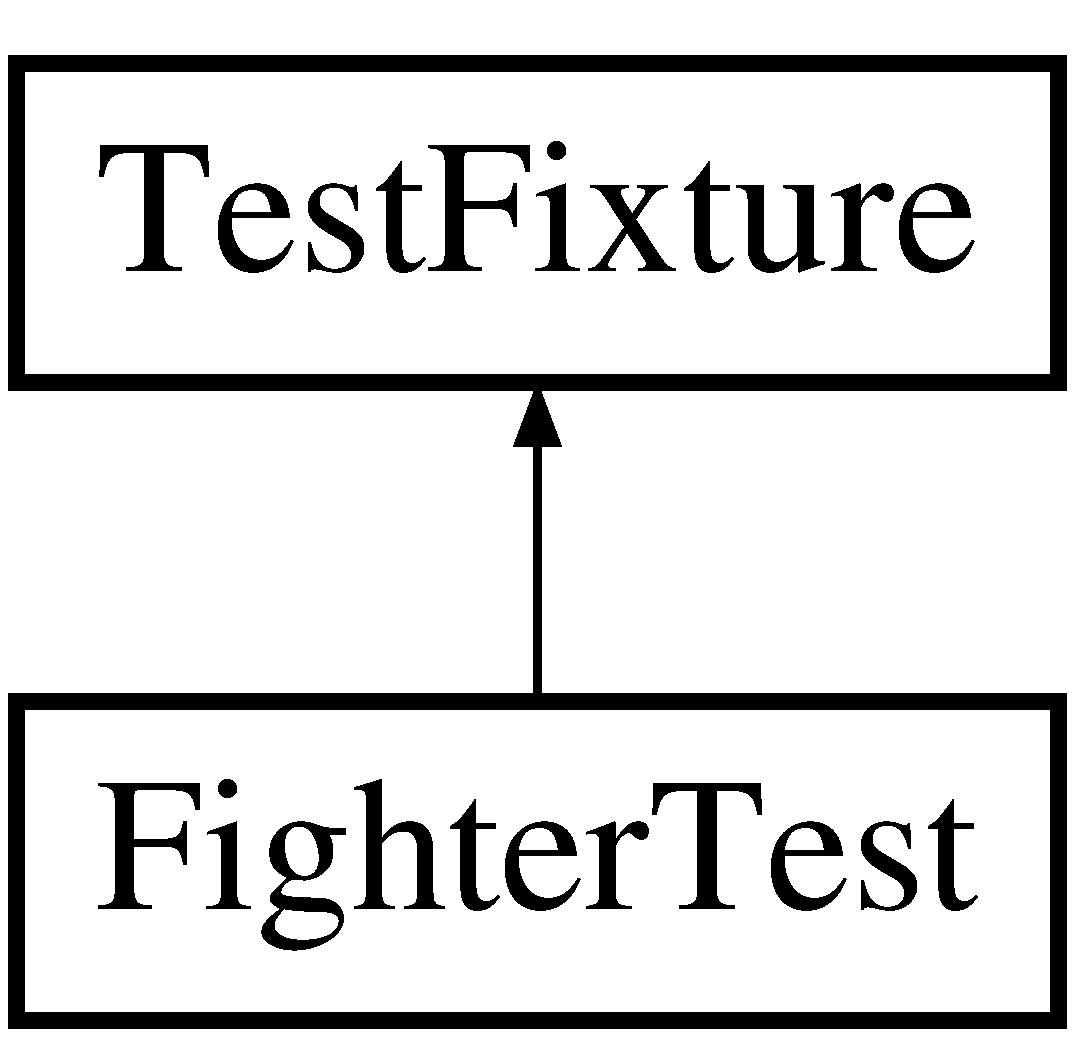
\includegraphics[height=2.000000cm]{class_fighter_test}
\end{center}
\end{figure}
\subsection*{Protected Member Functions}
\begin{DoxyCompactItemize}
\item 
\hypertarget{class_fighter_test_af0641c84ec71e42b396280ec853cb093}{}\label{class_fighter_test_af0641c84ec71e42b396280ec853cb093} 
void {\bfseries test\+Valid\+New\+Character} ()
\item 
\hypertarget{class_fighter_test_a3d0a319b2acbf2b30dfc8202e6a87e9e}{}\label{class_fighter_test_a3d0a319b2acbf2b30dfc8202e6a87e9e} 
void {\bfseries test\+Proficiency\+Bonus} ()
\item 
\hypertarget{class_fighter_test_a14379ceead9ab87e992abe1feb769117}{}\label{class_fighter_test_a14379ceead9ab87e992abe1feb769117} 
void \hyperlink{class_fighter_test_a14379ceead9ab87e992abe1feb769117}{test\+Valid\+Death} ()
\begin{DoxyCompactList}\small\item\em Test to validate if character dies when damage exceeds HP. \end{DoxyCompactList}\item 
\hypertarget{class_fighter_test_a3eb36e11675d352e3328fddbb9828a5f}{}\label{class_fighter_test_a3eb36e11675d352e3328fddbb9828a5f} 
void \hyperlink{class_fighter_test_a3eb36e11675d352e3328fddbb9828a5f}{test\+Valid\+Exp\+Gain} ()
\begin{DoxyCompactList}\small\item\em Test to validate if character exp gain from monster defeat is correct. \end{DoxyCompactList}\item 
void \hyperlink{class_fighter_test_a751fd0a97704e1101eb58f4493681696}{test\+Setting\+Fighter\+Position} ()
\end{DoxyCompactItemize}


\subsection{Detailed Description}
Test Class for the \hyperlink{class_fighter}{Fighter} class. 

\subsection{Member Function Documentation}
\hypertarget{class_fighter_test_a751fd0a97704e1101eb58f4493681696}{}\label{class_fighter_test_a751fd0a97704e1101eb58f4493681696} 
\index{Fighter\+Test@{Fighter\+Test}!test\+Setting\+Fighter\+Position@{test\+Setting\+Fighter\+Position}}
\index{test\+Setting\+Fighter\+Position@{test\+Setting\+Fighter\+Position}!Fighter\+Test@{Fighter\+Test}}
\subsubsection{\texorpdfstring{test\+Setting\+Fighter\+Position()}{testSettingFighterPosition()}}
{\footnotesize\ttfamily void Fighter\+Test\+::test\+Setting\+Fighter\+Position (\begin{DoxyParamCaption}{ }\end{DoxyParamCaption})\hspace{0.3cm}{\ttfamily [protected]}}

This test will ensure that setting the position of the \hyperlink{class_fighter}{Fighter} is working properly, and that new values of position can be retrieved accurently. 

The documentation for this class was generated from the following files\+:\begin{DoxyCompactItemize}
\item 
D\+:/\+Documents/\+A\+A\+S\+C\+H\+O\+O\+L/3-\/ Fall 2016/\+C\+O\+M\+P 345/\+Group Project/345dnd/\+Dand\+D/\hyperlink{_fighter_test_8cpp}{Fighter\+Test.\+cpp}\item 
D\+:/\+Documents/\+A\+A\+S\+C\+H\+O\+O\+L/3-\/ Fall 2016/\+C\+O\+M\+P 345/\+Group Project/345dnd/\+Dand\+D/Test\+Fighter\+Strategy.\+cpp\end{DoxyCompactItemize}

\hypertarget{class_helmet}{}\section{Helmet Class Reference}
\label{class_helmet}\index{Helmet@{Helmet}}


Class for helmets.  




{\ttfamily \#include $<$Helmet.\+h$>$}

Inheritance diagram for Helmet\+:\begin{figure}[H]
\begin{center}
\leavevmode
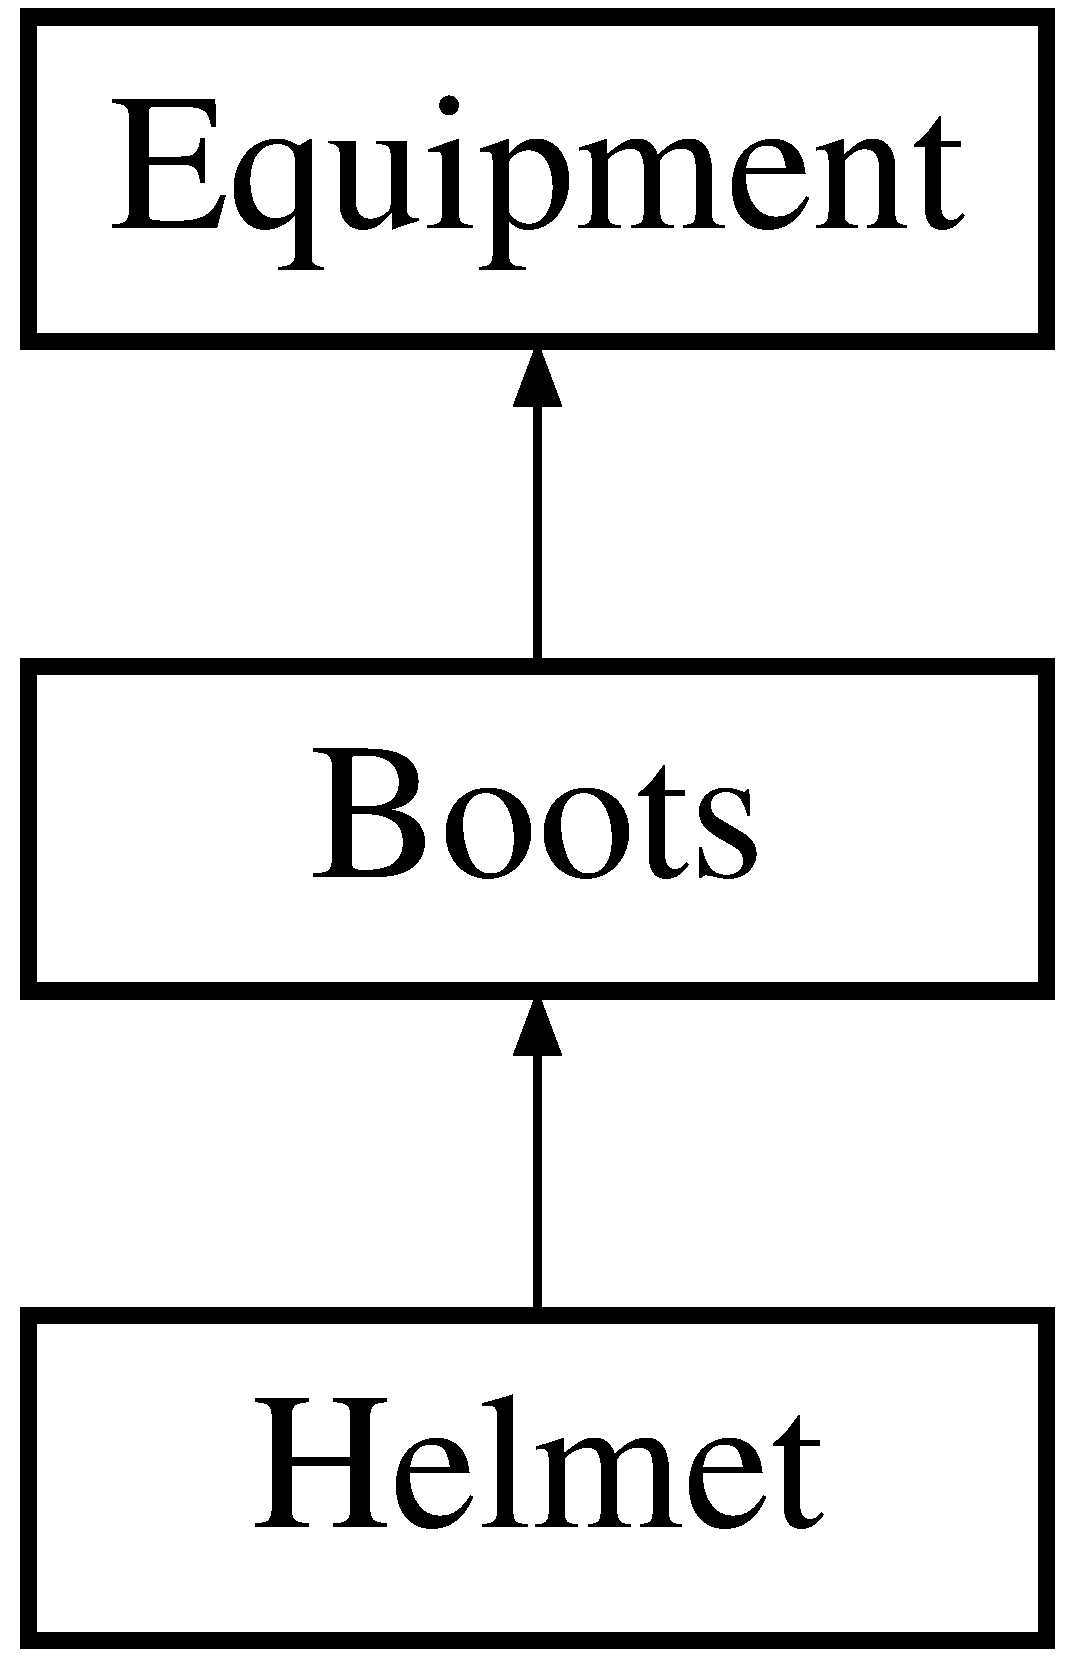
\includegraphics[height=3.000000cm]{class_helmet}
\end{center}
\end{figure}
\subsection*{Public Member Functions}
\begin{DoxyCompactItemize}
\item 
\hypertarget{class_helmet_ae9f39c8ca82962c770f9907123e663f5}{}\label{class_helmet_ae9f39c8ca82962c770f9907123e663f5} 
\hyperlink{class_helmet_ae9f39c8ca82962c770f9907123e663f5}{Helmet} ()
\begin{DoxyCompactList}\small\item\em Default constructor, useless item as is. \end{DoxyCompactList}\item 
\hyperlink{class_helmet_a27eceb089c04d2dcab69d49d30d7b92c}{Helmet} (const \hyperlink{class_helmet}{Helmet} $\ast$other\+Helmet)
\item 
\hypertarget{class_helmet_a53c7728aebd2aadb37082834cbec4968}{}\label{class_helmet_a53c7728aebd2aadb37082834cbec4968} 
{\bfseries Helmet} (string name, int weight, int value, string \hyperlink{class_item_add84a42b692ee5d580a92ae4a922f784}{image}, array$<$ int, 9 $>$ \hyperlink{class_item_a8532d8729f9433f41b7fc18b20d83236}{enchantment\+Values})
\item 
\hypertarget{class_helmet_abb01d02590723236e9cf9e260824e712}{}\label{class_helmet_abb01d02590723236e9cf9e260824e712} 
virtual void \hyperlink{class_helmet_abb01d02590723236e9cf9e260824e712}{Serialize} (C\+Archive \&ar)
\begin{DoxyCompactList}\small\item\em Allows \hyperlink{class_helmet}{Helmet} to be serialized. \end{DoxyCompactList}\item 
\hypertarget{class_helmet_afc4c216aed5d9402d9e33b95b1e2f9a3}{}\label{class_helmet_afc4c216aed5d9402d9e33b95b1e2f9a3} 
string {\bfseries to\+String} ()
\end{DoxyCompactItemize}
\subsection*{Protected Member Functions}
\begin{DoxyCompactItemize}
\item 
\hypertarget{class_helmet_a4d6756de7cf75e7cf04548c74d045ae2}{}\label{class_helmet_a4d6756de7cf75e7cf04548c74d045ae2} 
{\bfseries D\+E\+C\+L\+A\+R\+E\+\_\+\+S\+E\+R\+I\+AL} (\hyperlink{class_helmet}{Helmet})
\end{DoxyCompactItemize}
\subsection*{Additional Inherited Members}


\subsection{Detailed Description}
Class for helmets. 

\begin{DoxyAuthor}{Author}
Philip Brink 
\end{DoxyAuthor}
\begin{DoxyVersion}{Version}
0.\+0.\+1 
\end{DoxyVersion}
\begin{DoxyDate}{Date}
2016-\/10-\/20
\end{DoxyDate}
Subclass of \hyperlink{class_item}{Item}, allows Character to equip a helmet 

\subsection{Constructor \& Destructor Documentation}
\hypertarget{class_helmet_a27eceb089c04d2dcab69d49d30d7b92c}{}\label{class_helmet_a27eceb089c04d2dcab69d49d30d7b92c} 
\index{Helmet@{Helmet}!Helmet@{Helmet}}
\index{Helmet@{Helmet}!Helmet@{Helmet}}
\subsubsection{\texorpdfstring{Helmet()}{Helmet()}}
{\footnotesize\ttfamily Helmet\+::\+Helmet (\begin{DoxyParamCaption}\item[{const \hyperlink{class_helmet}{Helmet} $\ast$}]{other\+Helmet }\end{DoxyParamCaption})}

Copy-\/constructor -\/ initializes a new helmet to have the same values as another helmet 

The documentation for this class was generated from the following files\+:\begin{DoxyCompactItemize}
\item 
D\+:/\+Documents/\+A\+A\+S\+C\+H\+O\+O\+L/3-\/ Fall 2016/\+C\+O\+M\+P 345/\+Group Project/345dnd/\+Dand\+D/Helmet.\+h\item 
D\+:/\+Documents/\+A\+A\+S\+C\+H\+O\+O\+L/3-\/ Fall 2016/\+C\+O\+M\+P 345/\+Group Project/345dnd/\+Dand\+D/Helmet.\+cpp\end{DoxyCompactItemize}

\hypertarget{class_ring}{}\section{Ring Class Reference}
\label{class_ring}\index{Ring@{Ring}}


Class for rings.  




{\ttfamily \#include $<$Ring.\+h$>$}

Inheritance diagram for Ring\+:\begin{figure}[H]
\begin{center}
\leavevmode
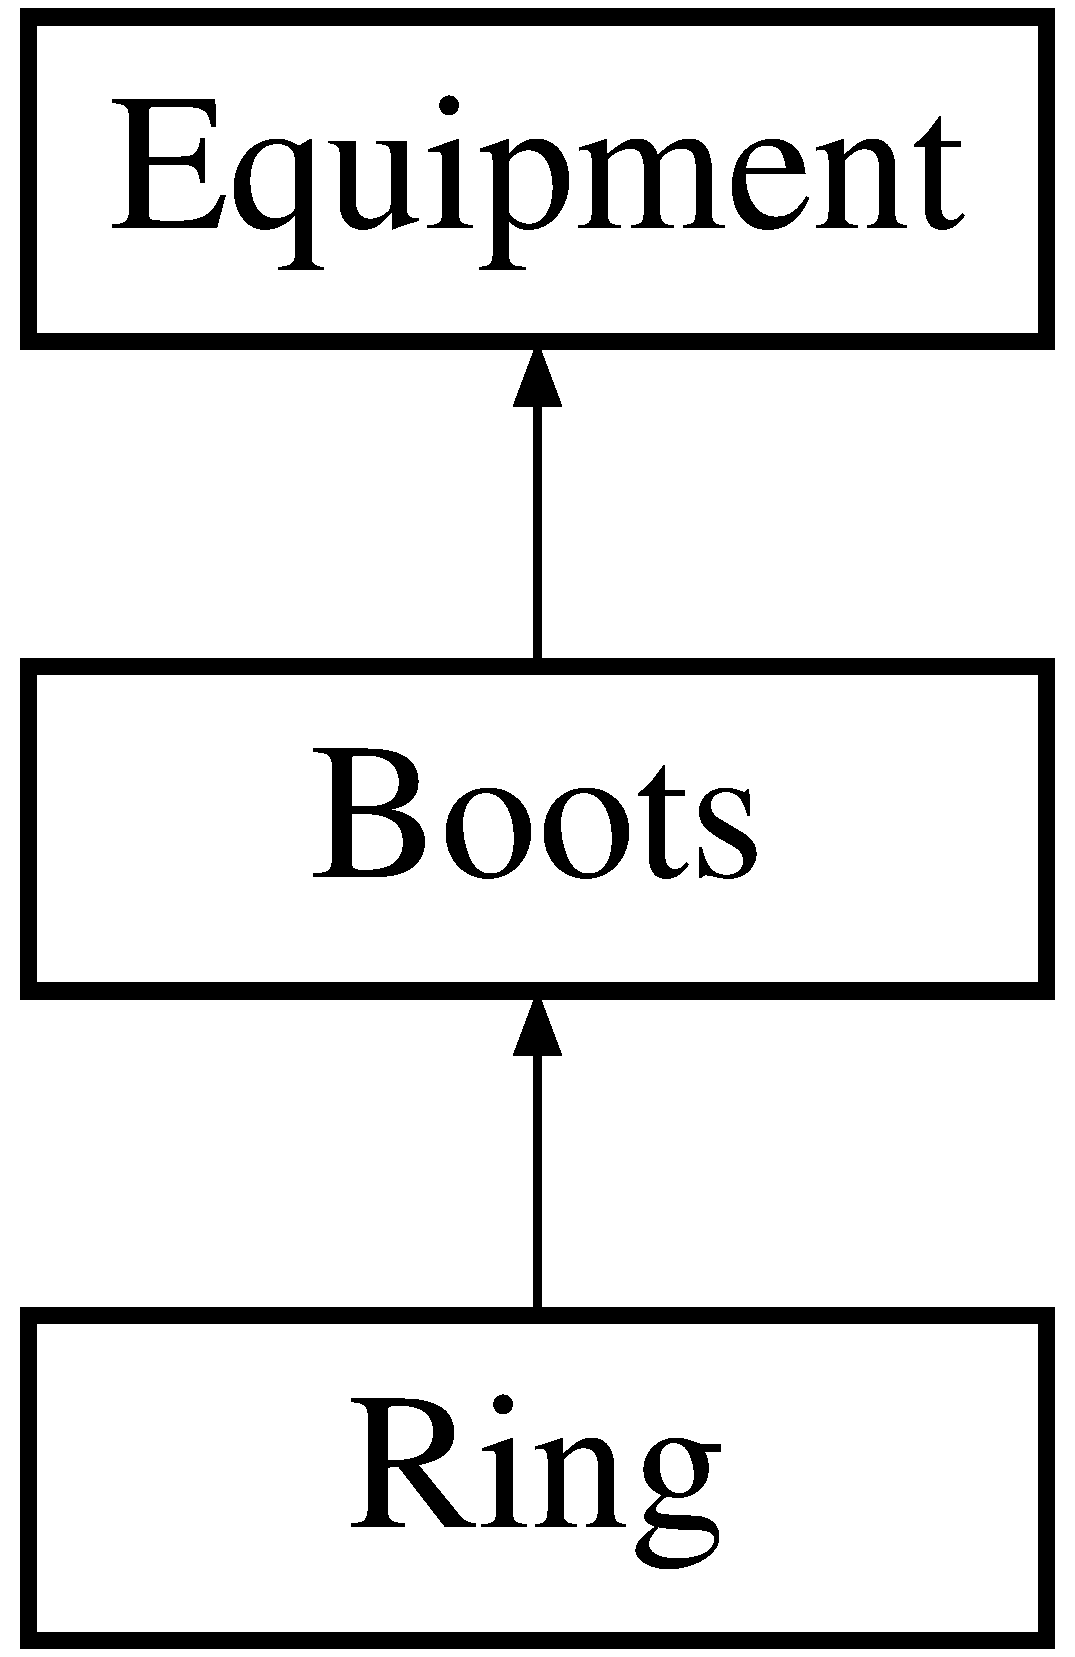
\includegraphics[height=3.000000cm]{class_ring}
\end{center}
\end{figure}
\subsection*{Public Member Functions}
\begin{DoxyCompactItemize}
\item 
\hyperlink{class_ring_ab65389fd4a0837c0f82a1b9207ba8330}{Ring} (const \hyperlink{class_ring}{Ring} $\ast$other\+Ring)
\item 
\hypertarget{class_ring_a0baf0ece716fa58742a031579310834b}{}\label{class_ring_a0baf0ece716fa58742a031579310834b} 
{\bfseries Ring} (string name, int weight, int value, string \hyperlink{class_item_add84a42b692ee5d580a92ae4a922f784}{image}, array$<$ int, 9 $>$ \hyperlink{class_item_a8532d8729f9433f41b7fc18b20d83236}{enchantment\+Values})
\item 
virtual void \hyperlink{class_ring_a123e40607e2aa46b27da2228af73eb4a}{Serialize} (C\+Archive \&ar)
\end{DoxyCompactItemize}
\subsection*{Protected Member Functions}
\begin{DoxyCompactItemize}
\item 
\hypertarget{class_ring_a46159bcedc7cf0fc72eec5d75784bed9}{}\label{class_ring_a46159bcedc7cf0fc72eec5d75784bed9} 
{\bfseries D\+E\+C\+L\+A\+R\+E\+\_\+\+S\+E\+R\+I\+AL} (\hyperlink{class_ring}{Ring})
\end{DoxyCompactItemize}
\subsection*{Additional Inherited Members}


\subsection{Detailed Description}
Class for rings. 

\begin{DoxyAuthor}{Author}
Philip Brink 
\end{DoxyAuthor}
\begin{DoxyVersion}{Version}
0.\+0.\+1 
\end{DoxyVersion}
\begin{DoxyDate}{Date}
2016-\/10-\/20
\end{DoxyDate}
Subclass of \hyperlink{class_item}{Item}, allows Character to equip a \hyperlink{class_ring}{Ring} 

\subsection{Constructor \& Destructor Documentation}
\hypertarget{class_ring_ab65389fd4a0837c0f82a1b9207ba8330}{}\label{class_ring_ab65389fd4a0837c0f82a1b9207ba8330} 
\index{Ring@{Ring}!Ring@{Ring}}
\index{Ring@{Ring}!Ring@{Ring}}
\subsubsection{\texorpdfstring{Ring()}{Ring()}}
{\footnotesize\ttfamily Ring\+::\+Ring (\begin{DoxyParamCaption}\item[{const \hyperlink{class_ring}{Ring} $\ast$}]{other\+Ring }\end{DoxyParamCaption})}

Copy Constructor -\/ runs the \hyperlink{class_item}{Item} copy constructor on the other ring object 

\subsection{Member Function Documentation}
\hypertarget{class_ring_a123e40607e2aa46b27da2228af73eb4a}{}\label{class_ring_a123e40607e2aa46b27da2228af73eb4a} 
\index{Ring@{Ring}!Serialize@{Serialize}}
\index{Serialize@{Serialize}!Ring@{Ring}}
\subsubsection{\texorpdfstring{Serialize()}{Serialize()}}
{\footnotesize\ttfamily void Ring\+::\+Serialize (\begin{DoxyParamCaption}\item[{C\+Archive \&}]{ar }\end{DoxyParamCaption})\hspace{0.3cm}{\ttfamily [virtual]}}

Allows an item to be serialized 

Reimplemented from \hyperlink{class_item_ad1eae21e57fc3ce3252080a4efbfb8e8}{Item}.



The documentation for this class was generated from the following files\+:\begin{DoxyCompactItemize}
\item 
Ring.\+h\item 
Ring.\+cpp\end{DoxyCompactItemize}

\hypertarget{class_shield}{}\section{Shield Class Reference}
\label{class_shield}\index{Shield@{Shield}}


Subclass of \hyperlink{class_item}{Item}, allows character to equip a \hyperlink{class_shield}{Shield}.  




{\ttfamily \#include $<$Shield.\+h$>$}

Inheritance diagram for Shield\+:\begin{figure}[H]
\begin{center}
\leavevmode
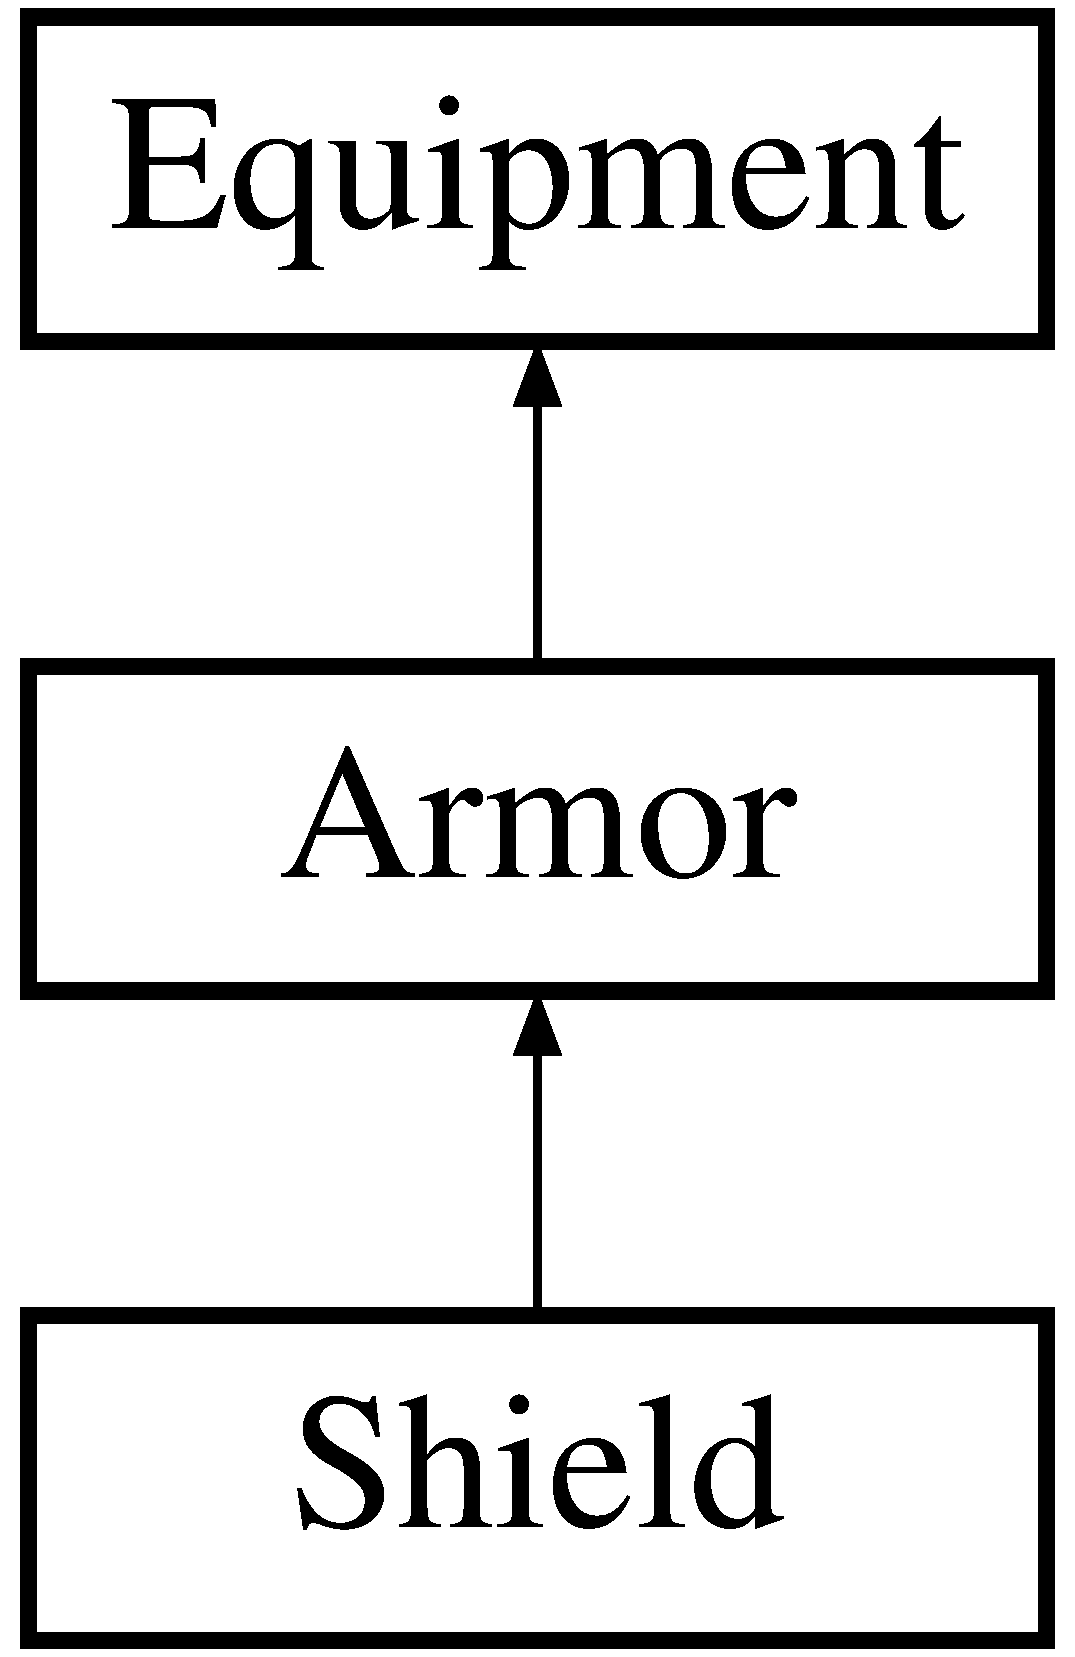
\includegraphics[height=3.000000cm]{class_shield}
\end{center}
\end{figure}
\subsection*{Public Member Functions}
\begin{DoxyCompactItemize}
\item 
\hypertarget{class_shield_a8a6e827c94750d8c1a1d523cb1b105de}{}\label{class_shield_a8a6e827c94750d8c1a1d523cb1b105de} 
\hyperlink{class_shield_a8a6e827c94750d8c1a1d523cb1b105de}{Shield} ()
\begin{DoxyCompactList}\small\item\em Default constructor, useless item as is. \end{DoxyCompactList}\item 
\hypertarget{class_shield_ae3dbea08547d4547faa441e5169605ba}{}\label{class_shield_ae3dbea08547d4547faa441e5169605ba} 
{\bfseries Shield} (string name, int weight, int value, string \hyperlink{class_item_add84a42b692ee5d580a92ae4a922f784}{image}, array$<$ int, 9 $>$ \hyperlink{class_item_a8532d8729f9433f41b7fc18b20d83236}{enchantment\+Values}, int defense, std\+::string attack\+Dice, int range)
\item 
\hypertarget{class_shield_a8c77767b623247b3ce1d42cbe3d3da05}{}\label{class_shield_a8c77767b623247b3ce1d42cbe3d3da05} 
{\bfseries Shield} (const \hyperlink{class_shield}{Shield} $\ast$other\+Shield)
\item 
\hypertarget{class_shield_a92fae272ca41b96a9f38770de4ed6180}{}\label{class_shield_a92fae272ca41b96a9f38770de4ed6180} 
int \hyperlink{class_shield_a92fae272ca41b96a9f38770de4ed6180}{get\+Defense} ()
\begin{DoxyCompactList}\small\item\em Gets defense of shield. \end{DoxyCompactList}\item 
\hypertarget{class_shield_a3e421a1c80aae934300dadf6db390bf1}{}\label{class_shield_a3e421a1c80aae934300dadf6db390bf1} 
void \hyperlink{class_shield_a3e421a1c80aae934300dadf6db390bf1}{set\+Defense} (int defense)
\begin{DoxyCompactList}\small\item\em Sets defense. \end{DoxyCompactList}\item 
\hypertarget{class_shield_a4031510f895e4163ee2b447d7992e08b}{}\label{class_shield_a4031510f895e4163ee2b447d7992e08b} 
void \hyperlink{class_shield_a4031510f895e4163ee2b447d7992e08b}{increment\+Defense} ()
\begin{DoxyCompactList}\small\item\em Increments defense. \end{DoxyCompactList}\item 
\hypertarget{class_shield_a90fe2bbca5c029c88715490c5525e1a6}{}\label{class_shield_a90fe2bbca5c029c88715490c5525e1a6} 
void \hyperlink{class_shield_a90fe2bbca5c029c88715490c5525e1a6}{decrement\+Defense} ()
\begin{DoxyCompactList}\small\item\em Decrements defense. \end{DoxyCompactList}\item 
\hypertarget{class_shield_a2e36b34d593ce4de9066c206c3528846}{}\label{class_shield_a2e36b34d593ce4de9066c206c3528846} 
void \hyperlink{class_shield_a2e36b34d593ce4de9066c206c3528846}{increment\+Range} ()
\begin{DoxyCompactList}\small\item\em Increments range. \end{DoxyCompactList}\item 
\hypertarget{class_shield_afeb7f31a542d80ededa37980f13df576}{}\label{class_shield_afeb7f31a542d80ededa37980f13df576} 
void \hyperlink{class_shield_afeb7f31a542d80ededa37980f13df576}{decrement\+Range} ()
\begin{DoxyCompactList}\small\item\em Decrements range. \end{DoxyCompactList}\item 
\hypertarget{class_shield_adca98dd6afb94104adbdadde591ae1e2}{}\label{class_shield_adca98dd6afb94104adbdadde591ae1e2} 
std\+::string {\bfseries get\+Attack\+Dice} ()
\item 
\hypertarget{class_shield_a69ddf60fb2bfe723051f535b8f1f5cd6}{}\label{class_shield_a69ddf60fb2bfe723051f535b8f1f5cd6} 
void {\bfseries set\+Attack\+Dice} (std\+::string attack\+Dice)
\item 
\hypertarget{class_shield_af8b6fccff0ddb7851440da08b4c76c8f}{}\label{class_shield_af8b6fccff0ddb7851440da08b4c76c8f} 
int \hyperlink{class_shield_af8b6fccff0ddb7851440da08b4c76c8f}{get\+Range} ()
\begin{DoxyCompactList}\small\item\em Gets range of shield. \end{DoxyCompactList}\item 
\hypertarget{class_shield_a7e0638047be589b3ab2ca0c1349f3409}{}\label{class_shield_a7e0638047be589b3ab2ca0c1349f3409} 
void \hyperlink{class_shield_a7e0638047be589b3ab2ca0c1349f3409}{set\+Range} (int range)
\begin{DoxyCompactList}\small\item\em Sets range of shield for attack. \end{DoxyCompactList}\item 
\hypertarget{class_shield_a524d5884f91f2539db047cecd09d6bc8}{}\label{class_shield_a524d5884f91f2539db047cecd09d6bc8} 
std\+::string {\bfseries to\+String} ()
\item 
virtual void \hyperlink{class_shield_a8d045c43b16aab5fc474e696cb8a7f1f}{Serialize} (C\+Archive \&ar)
\end{DoxyCompactItemize}
\subsection*{Protected Member Functions}
\begin{DoxyCompactItemize}
\item 
\hypertarget{class_shield_a0bc1e651aeb25fcecd483c76a847bb61}{}\label{class_shield_a0bc1e651aeb25fcecd483c76a847bb61} 
{\bfseries D\+E\+C\+L\+A\+R\+E\+\_\+\+S\+E\+R\+I\+AL} (\hyperlink{class_shield}{Shield})
\end{DoxyCompactItemize}
\subsection*{Protected Attributes}
\begin{DoxyCompactItemize}
\item 
\hypertarget{class_shield_af22e87b1ecaf100736797e30df248a8e}{}\label{class_shield_af22e87b1ecaf100736797e30df248a8e} 
int {\bfseries defense}
\item 
\hypertarget{class_shield_a4bcf1d65dc7b666ffc5ca465c37d98b9}{}\label{class_shield_a4bcf1d65dc7b666ffc5ca465c37d98b9} 
std\+::string {\bfseries attack\+Dice}
\item 
\hypertarget{class_shield_ad5c23fb3c974dd066b089a2841c4e2dd}{}\label{class_shield_ad5c23fb3c974dd066b089a2841c4e2dd} 
int {\bfseries range}
\end{DoxyCompactItemize}


\subsection{Detailed Description}
Subclass of \hyperlink{class_item}{Item}, allows character to equip a \hyperlink{class_shield}{Shield}. 

\subsection{Member Function Documentation}
\hypertarget{class_shield_a8d045c43b16aab5fc474e696cb8a7f1f}{}\label{class_shield_a8d045c43b16aab5fc474e696cb8a7f1f} 
\index{Shield@{Shield}!Serialize@{Serialize}}
\index{Serialize@{Serialize}!Shield@{Shield}}
\subsubsection{\texorpdfstring{Serialize()}{Serialize()}}
{\footnotesize\ttfamily void Shield\+::\+Serialize (\begin{DoxyParamCaption}\item[{C\+Archive \&}]{ar }\end{DoxyParamCaption})\hspace{0.3cm}{\ttfamily [virtual]}}

Allows an item to be serialized 

Reimplemented from \hyperlink{class_item_ad1eae21e57fc3ce3252080a4efbfb8e8}{Item}.



The documentation for this class was generated from the following files\+:\begin{DoxyCompactItemize}
\item 
\hyperlink{_shield_8h}{Shield.\+h}\item 
\hyperlink{_shield_8cpp}{Shield.\+cpp}\end{DoxyCompactItemize}

\hypertarget{class_weapon}{}\section{Weapon Class Reference}
\label{class_weapon}\index{Weapon@{Weapon}}


Subclass of \hyperlink{class_item}{Item}, allows character to equip a \hyperlink{class_weapon}{Weapon}.  




{\ttfamily \#include $<$Weapon.\+h$>$}

Inheritance diagram for Weapon\+:\begin{figure}[H]
\begin{center}
\leavevmode
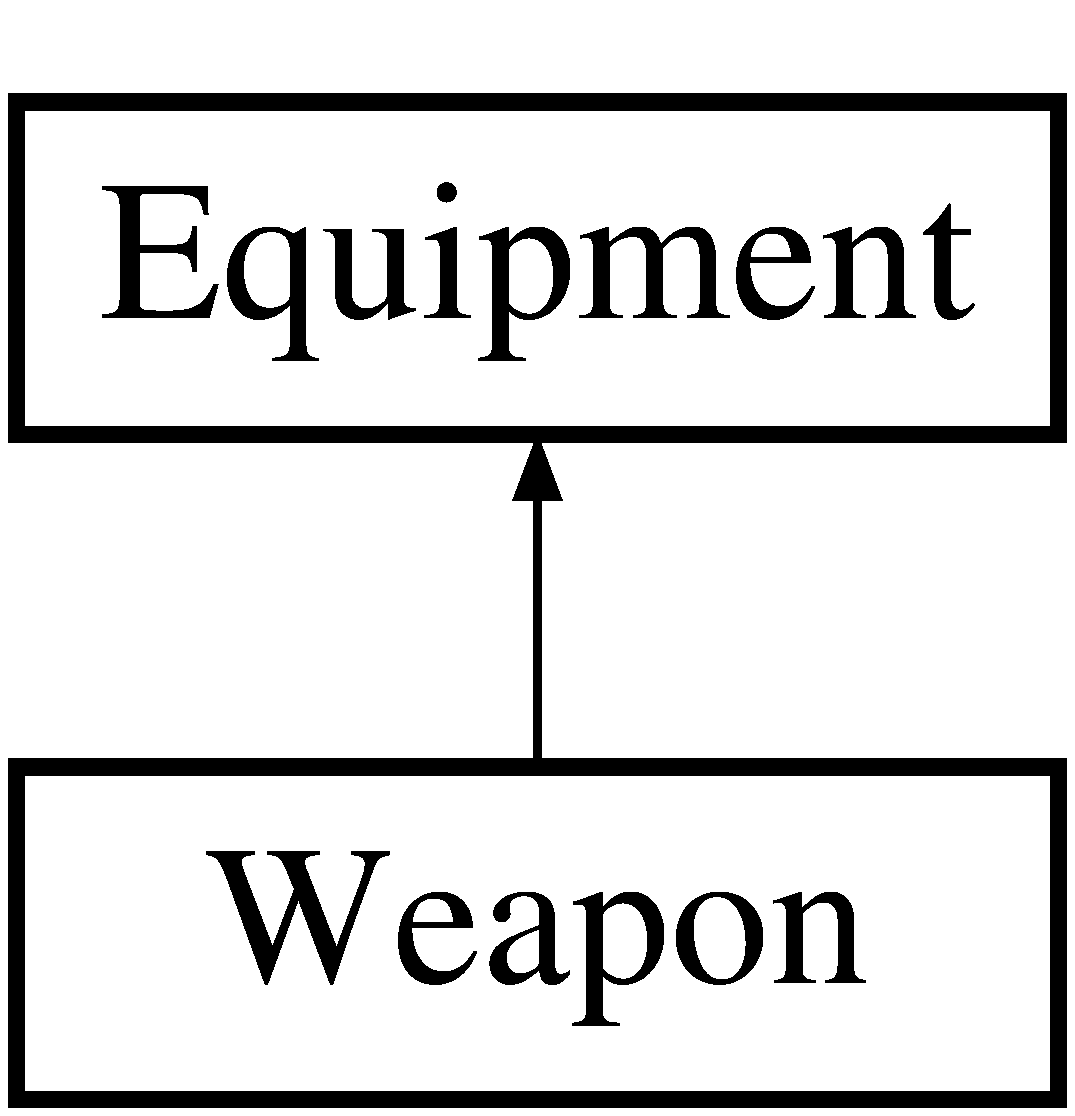
\includegraphics[height=3.000000cm]{class_weapon}
\end{center}
\end{figure}
\subsection*{Public Member Functions}
\begin{DoxyCompactItemize}
\item 
\hypertarget{class_weapon_ad948f8cbd8110949240e46c7c72c9556}{}\label{class_weapon_ad948f8cbd8110949240e46c7c72c9556} 
{\bfseries Weapon} (const \hyperlink{class_weapon}{Weapon} $\ast$other\+Weapon)
\item 
\hypertarget{class_weapon_a0fc6a57eb8c887a7e4a9d72dea29755c}{}\label{class_weapon_a0fc6a57eb8c887a7e4a9d72dea29755c} 
{\bfseries Weapon} (string name, int weight, int value, string \hyperlink{class_item_add84a42b692ee5d580a92ae4a922f784}{image}, array$<$ int, 9 $>$ \hyperlink{class_item_a8532d8729f9433f41b7fc18b20d83236}{enchantment\+Values}, string attack\+Dice, int range)
\item 
\hypertarget{class_weapon_ab3452fb4487ff88c46a4586cde0260cb}{}\label{class_weapon_ab3452fb4487ff88c46a4586cde0260cb} 
string {\bfseries get\+Attack\+Dice} ()
\item 
\hypertarget{class_weapon_a17ae76ac029507219ba18f6940b08258}{}\label{class_weapon_a17ae76ac029507219ba18f6940b08258} 
void {\bfseries set\+Attack\+Dice} (string attack\+Dice)
\item 
\hypertarget{class_weapon_af0d86939f16add54fc7ae87fea85ac21}{}\label{class_weapon_af0d86939f16add54fc7ae87fea85ac21} 
int {\bfseries get\+Range} ()
\item 
\hypertarget{class_weapon_a9227da33ba03135c9df353a91a7b0013}{}\label{class_weapon_a9227da33ba03135c9df353a91a7b0013} 
void {\bfseries set\+Range} (int range)
\item 
\hypertarget{class_weapon_a7dd6eff2cc572adb9bef4b985a255920}{}\label{class_weapon_a7dd6eff2cc572adb9bef4b985a255920} 
void {\bfseries increment\+Range} ()
\item 
\hypertarget{class_weapon_a6e28001720b8f43ee74f0ac7d3008ba5}{}\label{class_weapon_a6e28001720b8f43ee74f0ac7d3008ba5} 
void {\bfseries decrement\+Range} ()
\item 
\hypertarget{class_weapon_af1e10f75793cadcaec54a2ff96879312}{}\label{class_weapon_af1e10f75793cadcaec54a2ff96879312} 
std\+::string {\bfseries to\+String} ()
\item 
virtual void \hyperlink{class_weapon_a1c30e8f2add0a1aa8558cfbff13ad728}{Serialize} (C\+Archive \&ar)
\end{DoxyCompactItemize}
\subsection*{Protected Member Functions}
\begin{DoxyCompactItemize}
\item 
\hypertarget{class_weapon_acccf5cf3803e3ab7f63490e0d49c9abe}{}\label{class_weapon_acccf5cf3803e3ab7f63490e0d49c9abe} 
{\bfseries D\+E\+C\+L\+A\+R\+E\+\_\+\+S\+E\+R\+I\+AL} (\hyperlink{class_weapon}{Weapon})
\end{DoxyCompactItemize}
\subsection*{Protected Attributes}
\begin{DoxyCompactItemize}
\item 
\hypertarget{class_weapon_a034430020bc2fefd021253b49014c334}{}\label{class_weapon_a034430020bc2fefd021253b49014c334} 
string {\bfseries attack\+Dice}
\item 
\hypertarget{class_weapon_a13cc71a89d0cf076f58a040767682478}{}\label{class_weapon_a13cc71a89d0cf076f58a040767682478} 
int {\bfseries range}
\end{DoxyCompactItemize}


\subsection{Detailed Description}
Subclass of \hyperlink{class_item}{Item}, allows character to equip a \hyperlink{class_weapon}{Weapon}. 

\subsection{Member Function Documentation}
\hypertarget{class_weapon_a1c30e8f2add0a1aa8558cfbff13ad728}{}\label{class_weapon_a1c30e8f2add0a1aa8558cfbff13ad728} 
\index{Weapon@{Weapon}!Serialize@{Serialize}}
\index{Serialize@{Serialize}!Weapon@{Weapon}}
\subsubsection{\texorpdfstring{Serialize()}{Serialize()}}
{\footnotesize\ttfamily void Weapon\+::\+Serialize (\begin{DoxyParamCaption}\item[{C\+Archive \&}]{ar }\end{DoxyParamCaption})\hspace{0.3cm}{\ttfamily [virtual]}}

Allows an item to be serialized 

Reimplemented from \hyperlink{class_item_ad1eae21e57fc3ce3252080a4efbfb8e8}{Item}.



The documentation for this class was generated from the following files\+:\begin{DoxyCompactItemize}
\item 
\hyperlink{_weapon_8h}{Weapon.\+h}\item 
\hyperlink{_weapon_8cpp}{Weapon.\+cpp}\end{DoxyCompactItemize}

%--- End generated contents ---

% Index
\backmatter
\newpage
\phantomsection
\clearemptydoublepage
\addcontentsline{toc}{chapter}{Index}
\printindex

\end{document}
